%% 美赛模板:正文部分

\documentclass[12pt]{article}  % 官方要求字号不小于 12 号,此处选择 12 号字体

% 本模板不需要填写年份,以当前电脑时间自动生成
% 请在以下的方括号中填写队伍控制号
\usepackage[2306372]{easymcm}  % 载入 EasyMCM 模板文件
\problem{C}  % 请在此处填写题号
\usepackage{mathptmx}  % 这是 Times 字体,中规中矩 
%\usepackage{mathpazo}  % 这是 COMAP 官方杂志采用的更好看的 Palatino 字体,可替代以上的 mathptmx 宏包

\title{An MCM Paper Made by Team 2306372}  % 标题

% 如需要修改题头(默认为 MCM/ICM),请使用以下命令(此处修改为 MCM)
%\renewcommand{\contest}{MCM}

% 文档开始
\begin{document}

% 此处填写摘要内容
\begin{abstract}
In today's society, the game industry is booming and more and more people are participating in the game industry. Games have become part of everyone's life.So many games are so well made and so expensive that games are now known as the Ninth art.

The wordle this game, only five letters, simple game six speculation has attracted millions of people visit, hundreds of thousands of twitter to share every day.The popularity of the game has also attracted the attention of all sectors of society. The New York Times invited us to build a model to predict how the number of Wordle users changes and how word attributes influence the number of guesses and accuracy of users.

At the beginning, our team thought that the first question was very simple. We used \textbf{simple exponential fitting and Gaussian fitting} to complete the first question to predict the number of people on March 1st. And the fitting effect was very good. The number of people predicted by the simple exponential fitting on March 1 was 18,785, and the goodness of fit:
$R^2 = 0.9968$. 
The number of people predicted by the Gaussian fitting on March 1 is 13,914, and the goodness of fit:
$R^2 = 0.9892$.
But we later found out that all of the data was shared by Twitter users and not by all of the players. The idea of survivor bias immediately came to our  mind.Immediately decided to use SIRS(Susceptible, Exposed, Infectious, Recovered) model.And the outcome of SIRS model is 20,720.


For the solution of the second and third problems, we firstly constructed a model for problem 3 and using the model to evluate the distribution of problem 2.

\textbf{Very noteworthy, we found errors in the data! We corrected this based on data from Wrodle's official Twitter posts! Please see Model 1 for a more detailed version of the discovery process.}

For the problem 3 mopodel, we score for all the words from 0(min) to 1(max), we use the \textbf{hierarchy analysis, analysis of various factors} on the data given on the website.For all grade is divided into 5 sections (0-0.25), (0.25-0.30), (0.30-0.37), (0.37-0.7), (0.7-1.0) (divided according to the number of samples, each section of grade has the relatively same amount of words). For the given word EERIE we first calculate its score using the model we developed in the problem 3 to evaluate it to get a score, and see which grade section the score is in. And the corresponding proportion of 1,2,3,4,5,6,X fitted by normal distribution is the result we want.

At last the distribution we claculated is 1 try: 0\%, 2 tries:4\%, 3 tries 21\%, 4 tries 34\%, 5 tries24\%, 6 tries12\%, X 3\%.


After evaluating all the words, the cocorrelation coefficient between our evaluation system and the average number of tries can reach over 0.5, which is a strongly related. EERIE used the above evaluation system to get his relevant grade. His greade in our system is 0.6046, which is relatively a difficult word!




    % 美赛论文中无需注明关键字。若您一定要使用,
    % 请将以下两行的注释号 '%' 去除,以使其生效
     \vspace{5pt}
     \textbf{Keywords}: Exponential Fitting, Normal Distribution Fitting, Infection Model, Correlation Coefficient, Normalization, Analytic Hierarchy Process 

\end{abstract}

\maketitle  % 生成 Summary Sheet
\tableofcontents  % 生成目录


% 正文开始
\section{Introduction}
\subsection{Problem Background}
Wordle is a popular word-guessing game that took the internet by storm in February 2022. In the game, players must guess a five-letter word in six attempts or fewer by entering possible words and receiving feedback on how many letters are correct and in the right place. After a cursory search, we found that there are as many as 30,000 five-letter English words, and they cover all aspects of life. The inexhaustible question bank brings new game experiences for everyone. By analyzing the attributes of a word, we can rate the words and identify their difficulty. To better predict how the public will play wordle in the future.




\subsection{Literature Review}
  As a word guessing game released by New York Times, the analyses that we do on wordle contains not only the word in its database(we analyse the words themselves to get its grade in our system, find the corresponding difficulty level and predict the distribution of the tries it may appear), but also the social relations reflected in the game. Wordle is a time killing game. People can play in almost any of their spare time. This character make it integrated in people's life, those Tweets posted on Twitter, any social hotspot have great influence on the popularity of Wordle, which directly determins the user number and the percetage of players who played in hard mode. 

\subsection{Our work}


a.In the solution of problem 1, a chart was made according to 359 figures. After observing the shapes, exponential prediction and Gaussian prediction were used, and the fitting effect was very good. After we noticed the bold font for the tweet, we immediately discussed the SIRS model and the actual number of March 1 game players, so we nested the SRIS model for analysis, and the results were satisfactory.
    
    
b. In solving the second problem, we fully analyzed the 359 given data , and made statistics and classification. As for the attributes of words, we fully consider the influence of various attributes on the average number of guesses. We analyzed the nine factors: 


1.letter frequency;2.word frequency;3.whether there are repetitions letter;4 number of vowels;5.more than three repetitions;6.whether the word starts with a vowe;7.whether the word ends with a vowel;8.consecutive repetitions;9.social hot spots influence these nine factors. 


Found 1.Word Frequency 2.Letters Frequency 3.Multiple Occurrences of Letters 4.Vowels and Consonants 5.Social hot is the five most important factors that have a high correlation with the final results.
    
    
 c. We use the Analytic Hierarchy Process evaluation method to grade the difficulty of each word and form a complete evaluation system. When processing data, we adopted appropriate normalization method for different data types, made correlation analysis for each group of data, and formed the final evaluation system for the different sizes of influences produced by different influencing factors by adopting appropriate weighting method, and fully analyzed the situation of the word EERIE required at the end. Came up with our rating of the word.



\section{Preparation of the Models}
\subsection{Assumptions}
a. By making a line chart of 359 numbers in excel, we found that the overall trend was more consistent with Gaussian prediction and exponential prediction.

b. In the process of reading, we thought about the survivor bias and the impact of social networks like a disease is contagious, and then found that building an epidemic model may be a better choice.

c.A susceptible person is infected by an infected person, becomes infected, can be cured and becomes susceptible again, has temporary immunity, no incubation period. Take one day as the minimum time unit of the model. The total number of people is N, take the total number of people remains the same. The ratio of various groups to the total number of people at time t is denoted as s(t), i(t), r(t). The time t=0 at beginning, the initial ratio of the number of all types of people is $s_0, i_0, r_0$. The daily exposure number $\gamma$ is the average number of susceptible persons who are effectively exposed to each infected person per day. The daily cure rate is $\mu$. Daily immunity loss is $\gamma$.

\subsection{Notations}
The primary notations used in this paper are listed in Table \ref{tb:notations}.

\begin{table}[!htbp]
	\begin{center}
		\caption{Notations}
		\begin{tabular}{cl}
			\toprule
			\multicolumn{1}{m{3cm}}{\centering Notation}
			&\multicolumn{1}{m{8cm}}{\centering Meaning}\\
			\midrule
			$ a,b,c,d $ &   \qquad\qquad\qquad the coefficient of Exp prediction\\
			$ a_1, b_1, c_1, a_2, b_2, c_2 $ &   \qquad\qquad\qquad the coefficient of Gauss prediction \\
			$SSE$ &  \qquad\qquad\qquad  the Sum of Squares due to Error\\
			$S (Susceptible)$&   \qquad\qquad\qquad Infection after contact with an infected person\\
			$I (Infectious)$&   \qquad\qquad\qquad A patient who can infect others\\
			$R (Recovered)$ &  \qquad\qquad\qquad  Recover from the disease, but can still be infected\\
			$N$& \qquad\qquad\qquad the total people\\
			$S(t) I(t) R(t)$& \qquad\qquad\qquad the number of three kinds of people\\
			$\lambda$& \qquad\qquad\qquad daily contact rate\\
			$\mu$& \qquad\qquad\qquad daily recovery rate\\
			$\gamma$& \qquad\qquad\qquad daily losing immune rate\\
			$R^{2}$& \qquad\qquad\qquad correlation coefficient\\
			$Ad justed R^{2}$& \qquad\qquad\qquad Ad justed correlation coefficient\\
			$RMSE$& \qquad\qquad\qquad Root Mean Square Error\\
			\bottomrule
		\end{tabular}\label{tb:notations}
	\end{center}
\end{table}


\clearpage
\section{The Models}
\subsection{Model 1}
\subsubsection{Exp prediction and Gaussian prediction}
The detail can be described by equation :

\begin{equation}
\large f(x)=a\cdot  e^{bx}+c\cdot e^{dx}
\end{equation}

$$Coefficient(Confidence \quad bounds: 95\%)$$
\begin{table}[!htbp]
	\begin{center}
		\caption{Exp prediction}
		\begin{tabular}{cl}
			\toprule
			\multicolumn{1}{m{3cm}}{\centering Formula}
			&\multicolumn{1}{m{8cm}}{\centering Range}\\
			\midrule
			$ a=7.07\times 10^{5}$ &   \qquad\qquad $(6.83\times 10^{5}, 7.309\times10^{5})$\\
			$ b=-0.02465 $ &   \qquad\qquad $(-0.02556, -0.02375)$\\
			$ c=6.184\times 10^{4}$ &  \qquad\qquad  $(5.503\times 10^{4}, 6.864\times 10^{4})$\\
			$ d$ &  \qquad\qquad  -0.002846(-0.003236,-0.002457)\\
			$ SSE$ &  \qquad\qquad  $1.0324\times 10^{10}$\\
			\bottomrule
		\end{tabular}\label{tb:notation}
	\end{center}
\end{table}

\begin{equation}
\large f(x) =  a_1\cdot e^{-\frac{x-b_1}{c_1}^2} + a_2\cdot e^{-\frac{x-b_2}{c_2}^2}
\end{equation}

$$Coefficient(Confidence bounds: 95\%)$$

\begin{table}[!htbp]
	\begin{center}
		\caption{Gauss prediction}
		\begin{tabular}{cl}
			\toprule
			\multicolumn{1}{m{3cm}}{\centering Formula}
			&\multicolumn{1}{m{8cm}}{\centering Range}\\
			\midrule
			$a1 =  1.014\times 10^{18} $&   \qquad\qquad$(-7.45\times 10^{20}, 7.47\times 10^{20})$\\
			$b1 =  -2997$&   \qquad\qquad $(-8.057\times 10^{4}, 7.457\times 10^{4})$\\
			$c1 =  565.3$ &  \qquad\qquad  (-6672, 7803)\\
			$a2 =  2.748\times 10^{4}$&   \qquad\qquad $(6742, 4.822\times 10^{4})$\\
			$b2 =  244 $&   \qquad\qquad (34.64, 453.3)\\
			$c2 =  210.6$ &  \qquad\qquad  (-14.9, 436.1)\\
			$SSE$ &  \qquad\qquad $1.0098\times 10^{10}$\\
			\bottomrule
		\end{tabular}\label{tb:notation}
	\end{center}
\end{table}


\begin{figure}[htbp]
	
	\begin{subfigure}[b]{.5\textwidth}
		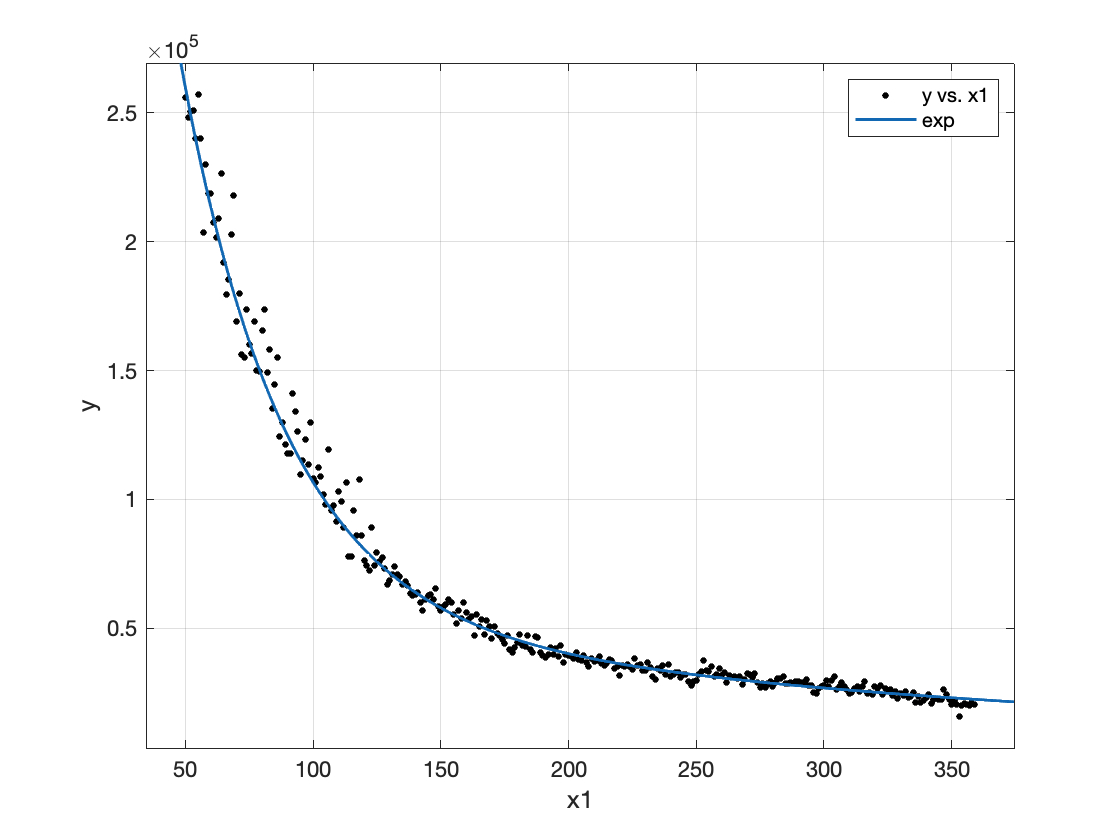
\includegraphics[width=\textwidth]{exp.jpg}
		\caption{Exp prediction}\label{subfig:left}
	\end{subfigure}
	\begin{subfigure}[b]{.5\textwidth}
		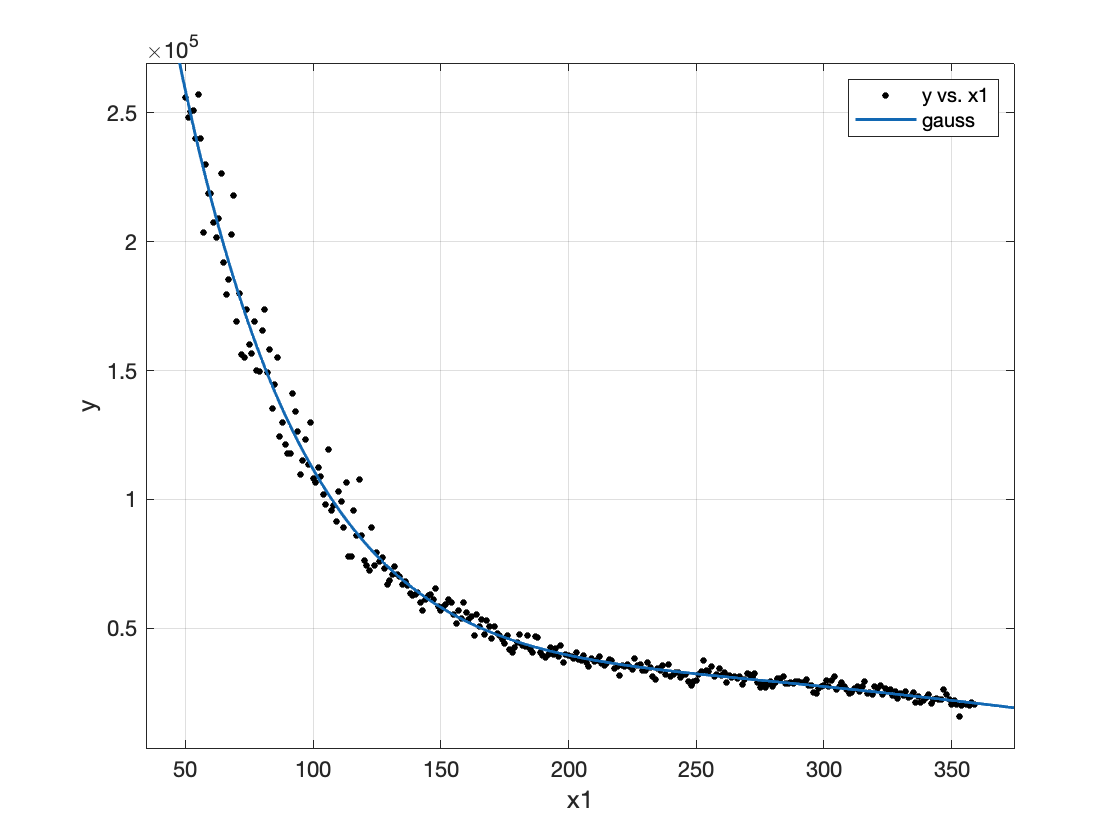
\includegraphics[width=\textwidth]{gauss.jpg}
		\caption{Gaussian predicition}\label{subfig:right}
	\end{subfigure}
	\caption{The outcome }\label{fig:subfigures}
	\end{figure}



The Trust-Region algorithm is used to calculate the number of users on March 1st. The estimated number of people playing Wordle games on March 1st is 18,785 according to Exp prediction, and the estimated number of people playing Wordle games on March 1st is 13,914 according to Gauss prediction. After our comparative analysis, we find that the 18,785 predicted by Exp is significantly more in line with the actual results. The Exp prediction model is suitable for those whose changes in the second half are in line with its function characteristics, but it cannot predict the results of the first half very well, because in the actual situation, the number of people playing Wordle games does not conform to the characteristics of the exponential function in the first half. The Gauss prediction can predict the whole segment, but the fitting degree is not ideal. Since we're predicting the number of players on March 1st, which is the second half of the function, we choose Exp, which predicts 18,785 players on March 1st.\\

\subsubsection{Improve:SIRS Model}
We used the SIRS \cite{1} model to simulate Wordle's model, and the population was roughly divided into three categories: susceptible population, diseased population, and recovered population.Corresponding to the game, population is the Wordle game, and enjoy their achievement to twitter.We think that others in the propaganda of the game to the society, they can be seen as a kind of contagion.And the susceptible population is people who never play the game and people who play the game but don't tweet .As for the rehabilitation population, it is people who play the game but give up playing the game and think they will not play the game in the future.After this connection was established, our team decided that we could use the SIRS model to predict the number of users on March 1st.Effect should be better than the Exp prediction and Gauss prediction.


\begin{figure}[htbp]
	\centering
	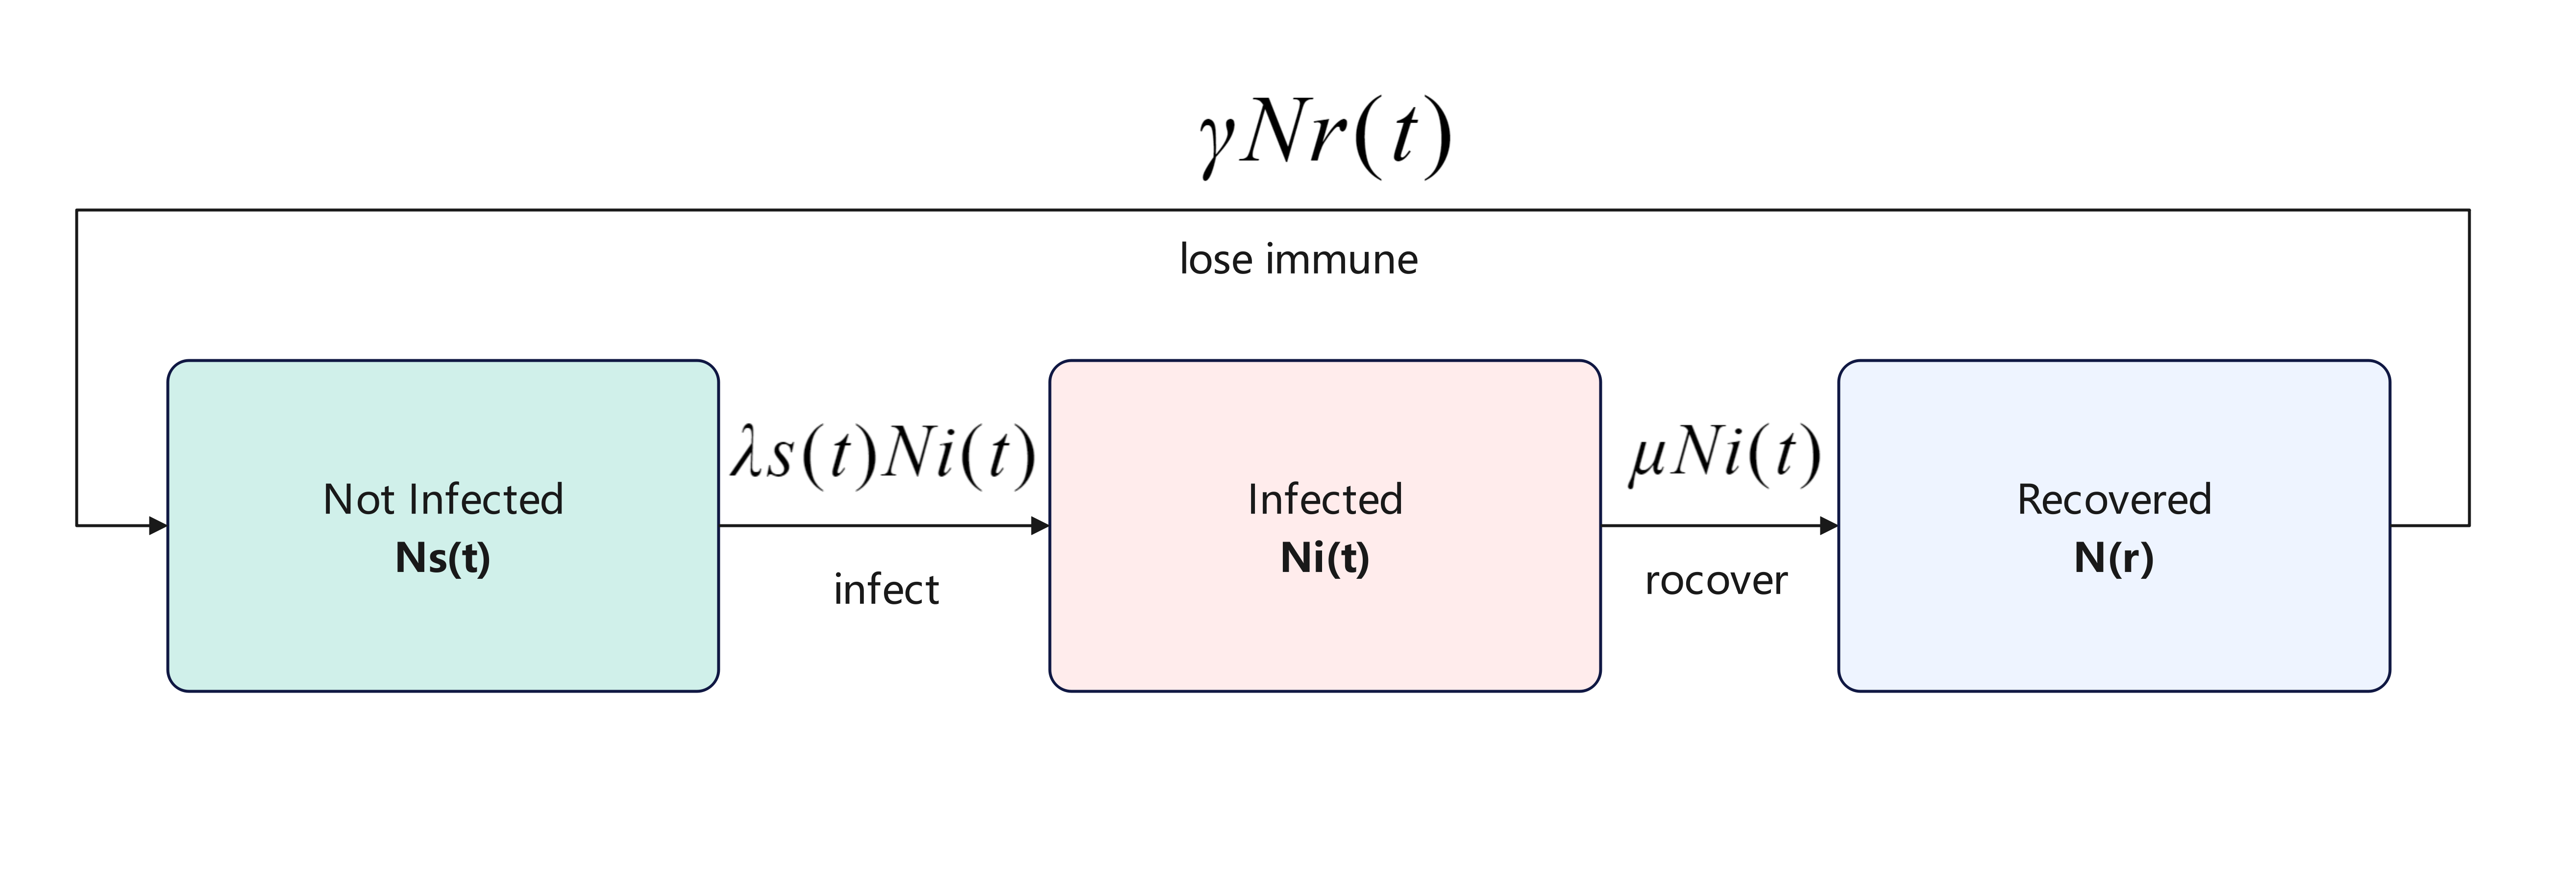
\includegraphics[width=0.9\textwidth]{1.jpg}
	\caption{SIRS Model}\label{fig:result}
\end{figure}



Considering that the spread of games is very similar to the spread of infectious diseases,we came up with the idea of using the model of infectious diseases to study this problem.
It is suitable for susceptible people, sick people and recovered people. Recovered people only have temporary immunity. People who become susceptible after unit time are likely to be infected again and get sick.



\subsubsection{Assumptions of SIRS Model}
A susceptible person is infected by effective contact with an infected person, becomes infected, can be cured and becomes susceptible again, has temporary immunity, no incubation period. Take one day as the minimum time unit of the model. The total number of people is N, regardless of the birth and death of the population, migration and migration, the total number of people remains the same. The ratio of various groups to the total number of people at time t is denoted as s(t), i(t), r(t) respectively, and the number of various groups is S(t), I(t), R(t). When the initial time t=0, the initial ratio of the number of all types of people is $s_0, i_0, r_0$. The daily exposure number $\gamma$ is the average number of susceptible persons who are effectively exposed to each infected person per day. The daily cure rate is $\mu$. that is, the ratio of the number of patients cured per day to the total number of patients. The average cure day is $\frac{1}{\mu}$. Also known as the average infection period, that is, the number of days from illness to cure. The infectious period contact number $\sigma=\frac{\gamma}{\mu}$is the number of susceptible persons effectively exposed to each infected person within $\frac{1}{\mu}$day of the entire infectious period. Daily immunity loss $\gamma$ is the percentage of the total number of rehabilitated persons who lose immunity each day.


\begin{table}[!htbp]
	\begin{center}
		\caption{The  SRIS Model}
		\begin{tabular}{cl}
			\toprule
			\multicolumn{1}{m{2cm}}{\centering Symbol}
			&\multicolumn{1}{m{8cm}}{\centering Meaning}\\
			\midrule
			$S (Susceptible)$&   \qquad\qquad\qquad Infection after contact with an infected person\\
			$I (Infectious)$&   \qquad\qquad\qquad A patient who can infect others\\
			$R (Recovered)$ &  \qquad\qquad\qquad  Recover from the disease, but can still be infected\\
			\bottomrule
		\end{tabular}\label{tb:notation}
	\end{center}
\end{table}

\begin{figure}[htbp]
	\centering
	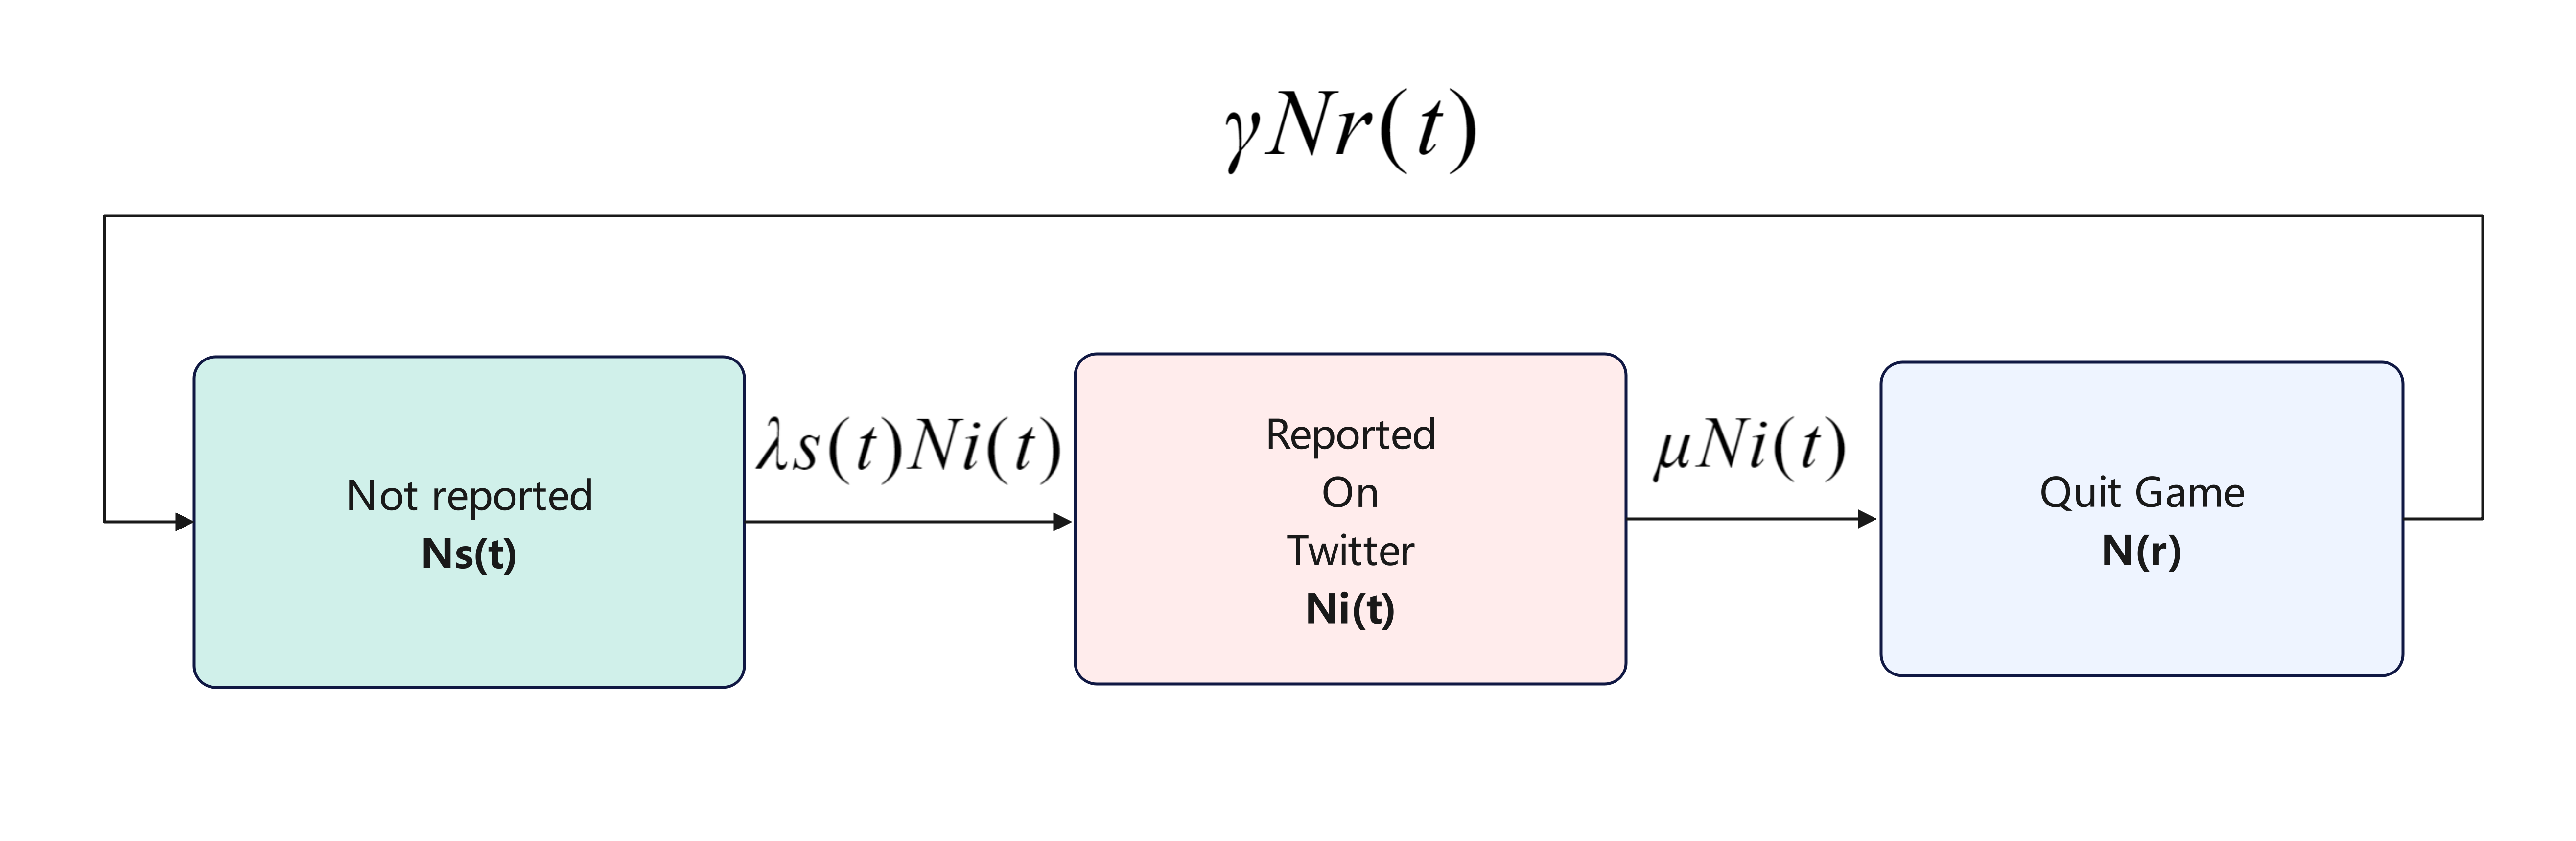
\includegraphics[width=0.9\textwidth]{2.jpg}
	\caption{New Model}\label{fig:result}
\end{figure}

As shown in the figure above, each patient can make $\lambda s(t)$ a susceptible person become infected, and the number of patients is $ N i(t)$, so there are $\lambda s(t) N i(t)$ a susceptible person infected every day, that is, the number of new patients every day.
Out of $ N i(t)$, $\mu n  i(t)$ is cured every day.
In the $Nr(t)$ of daily recoveries, $ \gamma N r(t)$ loses immunity and becomes susceptible.
The differential equation can be obtained:

\begin{equation}
\large N\frac{ds(t)}{dt} =-\lambda N\cdot s(t)i(t)+\gamma N\cdot r(t)
\end{equation}

\begin{equation}
\large N\frac{di(t)}{dt} =\lambda N\cdot s(t)i(t)-\mu N\cdot i(t)
\end{equation}

\begin{equation}
\large N\frac{dr(t)}{dt} =\mu N\cdot i(t)-\gamma N\cdot r(t)
\end{equation}

\begin{figure}[htbp]
	\centering
	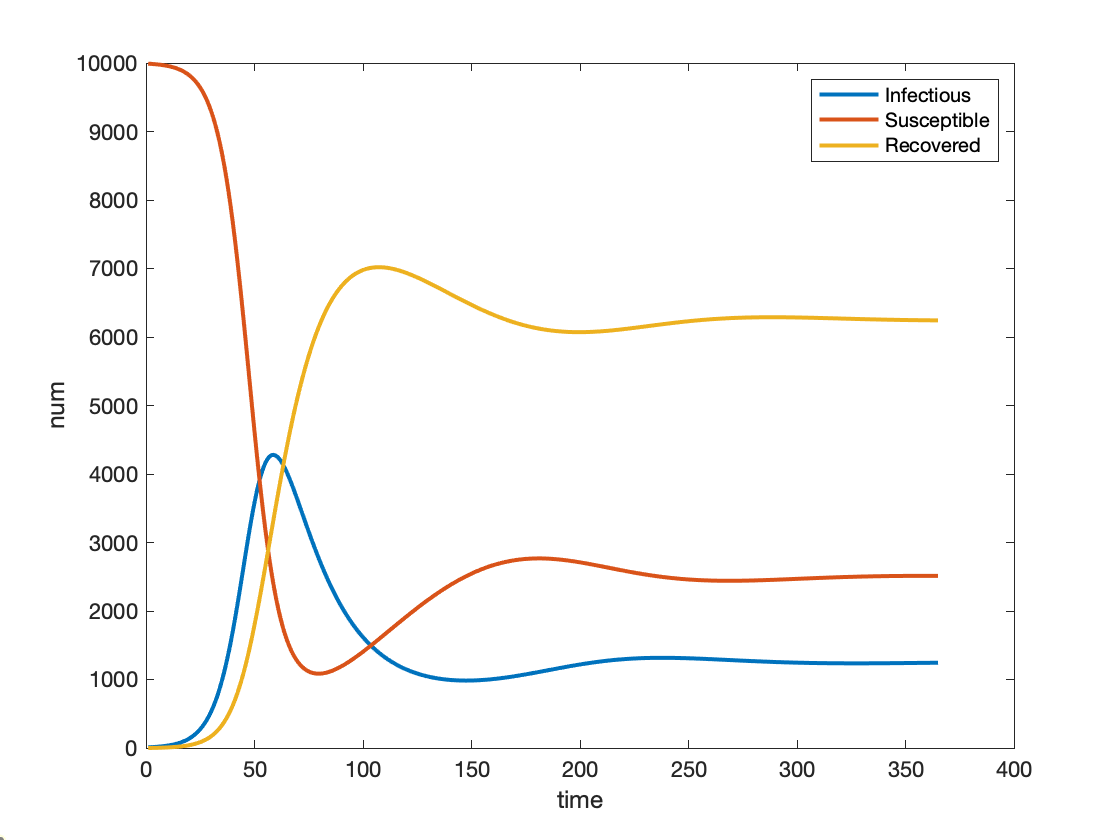
\includegraphics[width=0.9\textwidth]{SRIS1.jpg}
	\caption{SRIS Model}\label{fig:result}
\end{figure}



Let's look at the practical application of the model in this problem:
S represents the group of people who are likely to play the game or are already playing the game but are not tweeting.
I stands for the person who is playing the game and has already tweeted, after which more S can play the game and tweet.
R is the people who played the game and lost interest, but over time these people will become S, the probability of continuing to play the game.
Based on the calculation of the model and the actual data, we assume that the starting number of tweets S (0) is 84,000 (the starting number is not 0 because the data given is not the data from the beginning of the game), the starting number of tweets R (0) is 0, and the total number of tweets N is 525,000.


\begin{table}[!htbp]
	\begin{center}
		\caption{The  SRIS Model}
		\begin{tabular}{cl}
			\toprule
			\multicolumn{1}{m{2cm}}{\centering Symbol}
			&\multicolumn{1}{m{6cm}}{\centering Numerical value}\\
			\midrule
		\cr${\gamma}$&   \qquad\qquad\qquad\qquad 0.17\%\\
		\cr${\mu}$&   \qquad\qquad\qquad\qquad 2\%\\
		\cr${\lambda}$ &  \qquad\qquad\qquad \qquad 11\%\\
		\cr$SSE$ &  \qquad\qquad\qquad \qquad $1.4889\times 10^{10}$\\
			\bottomrule
		\end{tabular}\label{tb:notation}
	\end{center}
\end{table}

By substituting the above differential equation and programming simulation, the following results are obtained:

\begin{figure}[htbp]
	\centering
	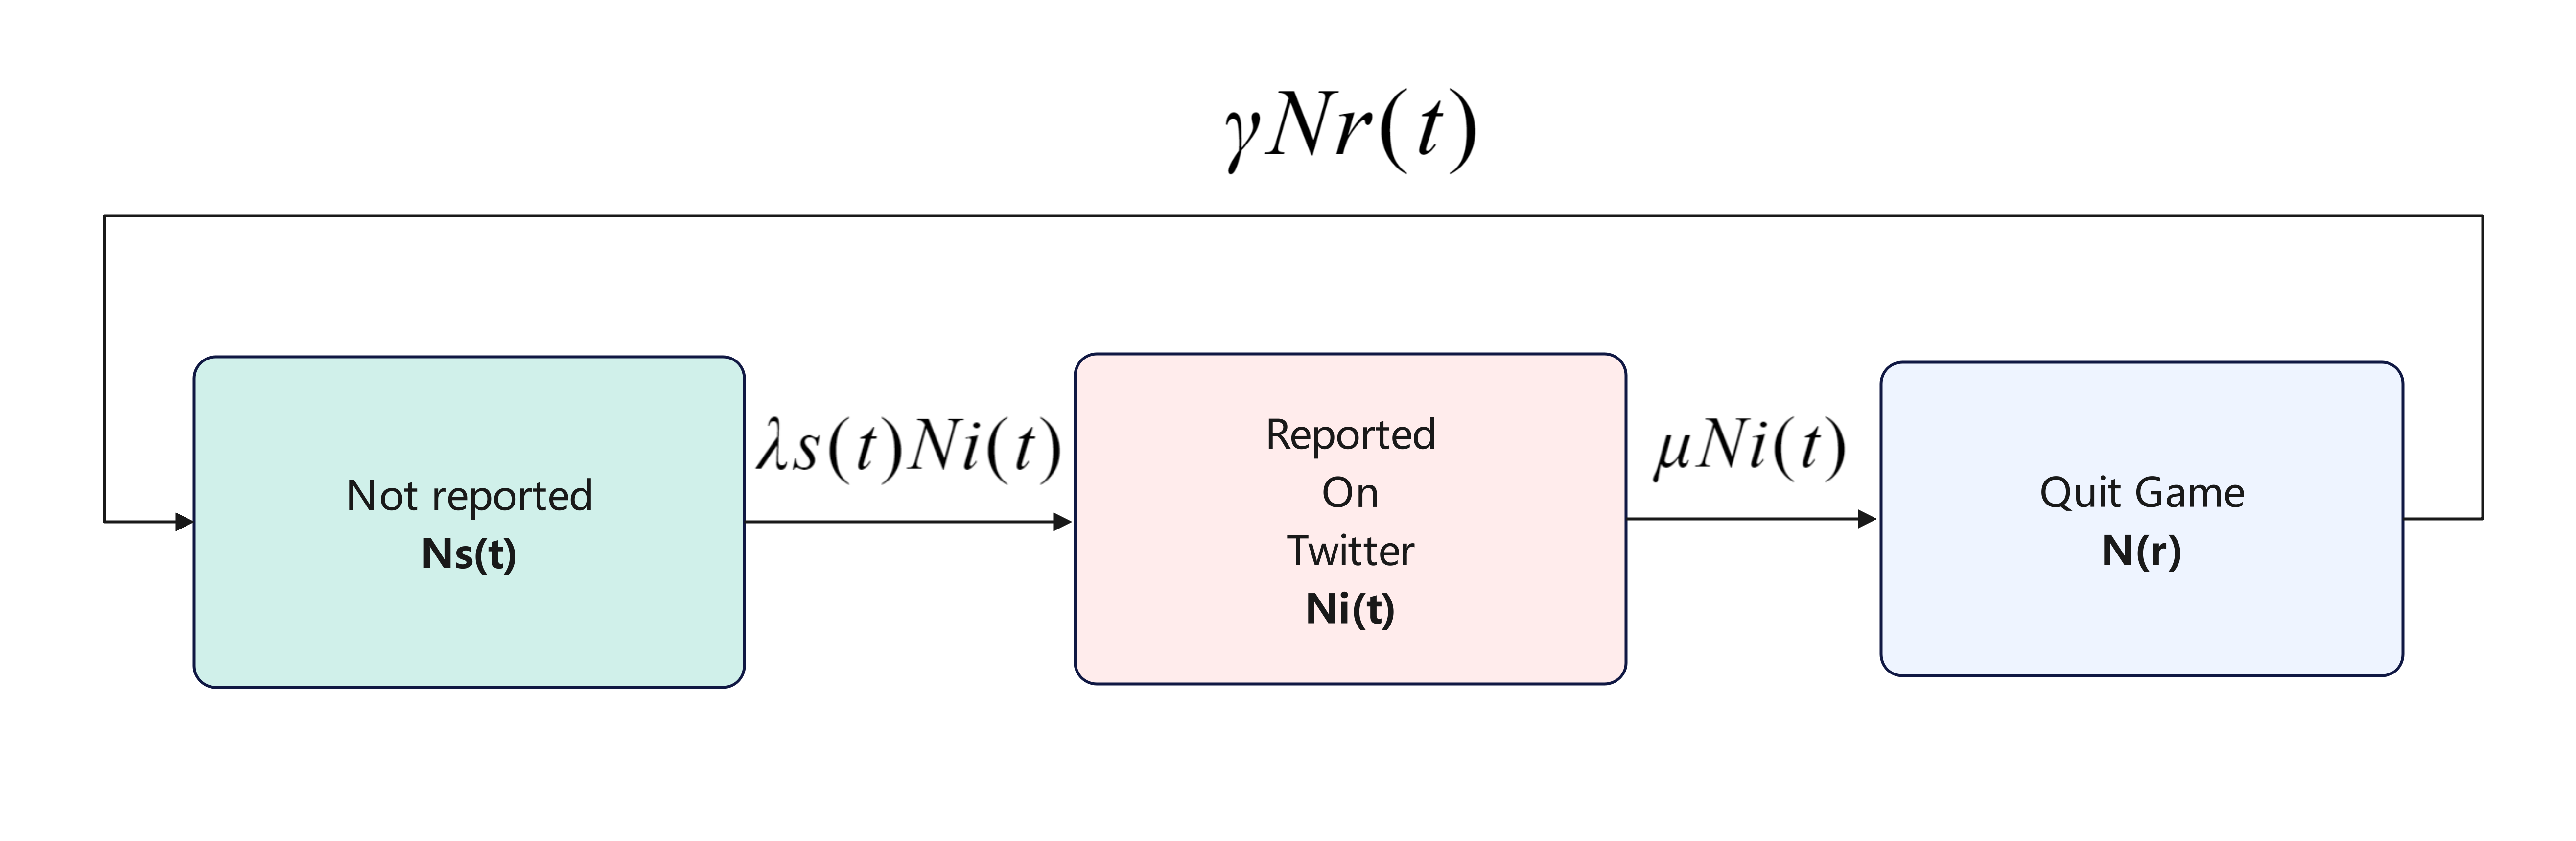
\includegraphics[width=0.7\textwidth]{2.jpg}
	\caption{New Model}\label{fig:result}
\end{figure}

\begin{figure}[htbp]
	
	\begin{subfigure}[b]{.5\textwidth}
		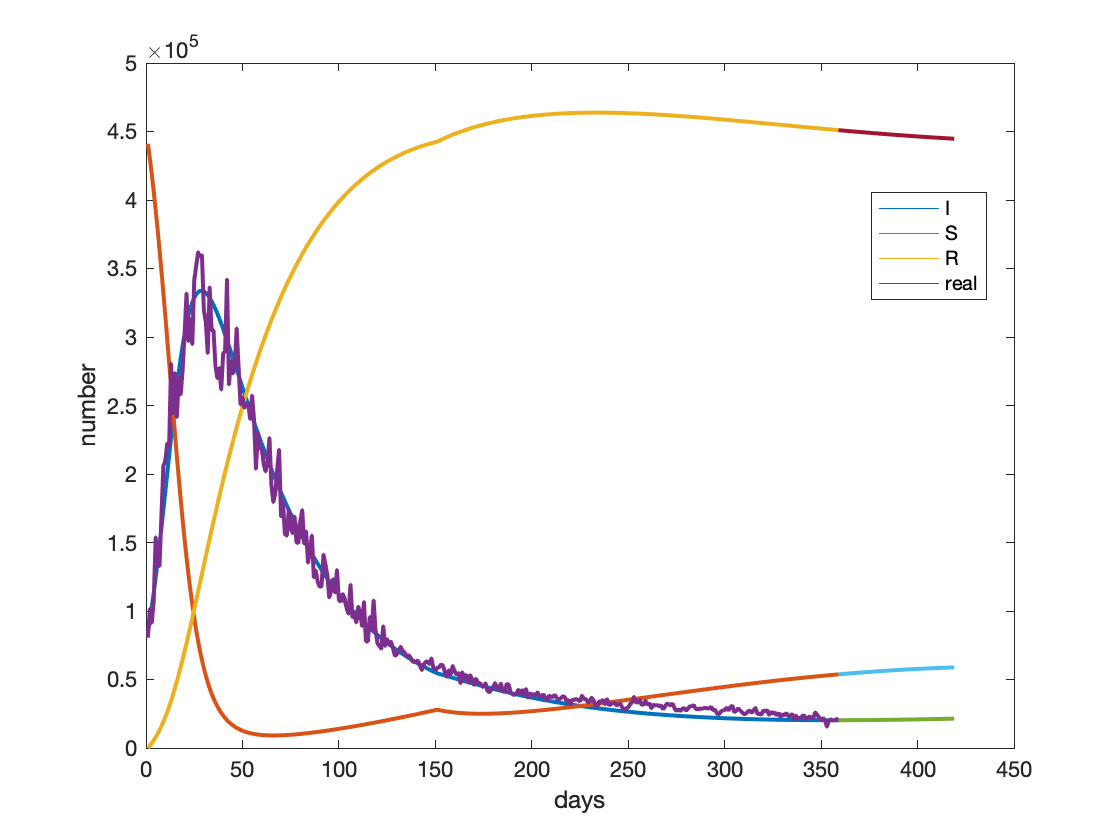
\includegraphics[width=\textwidth]{SRIS2.jpg}
		
	\end{subfigure}
	\begin{subfigure}[b]{.5\textwidth}
		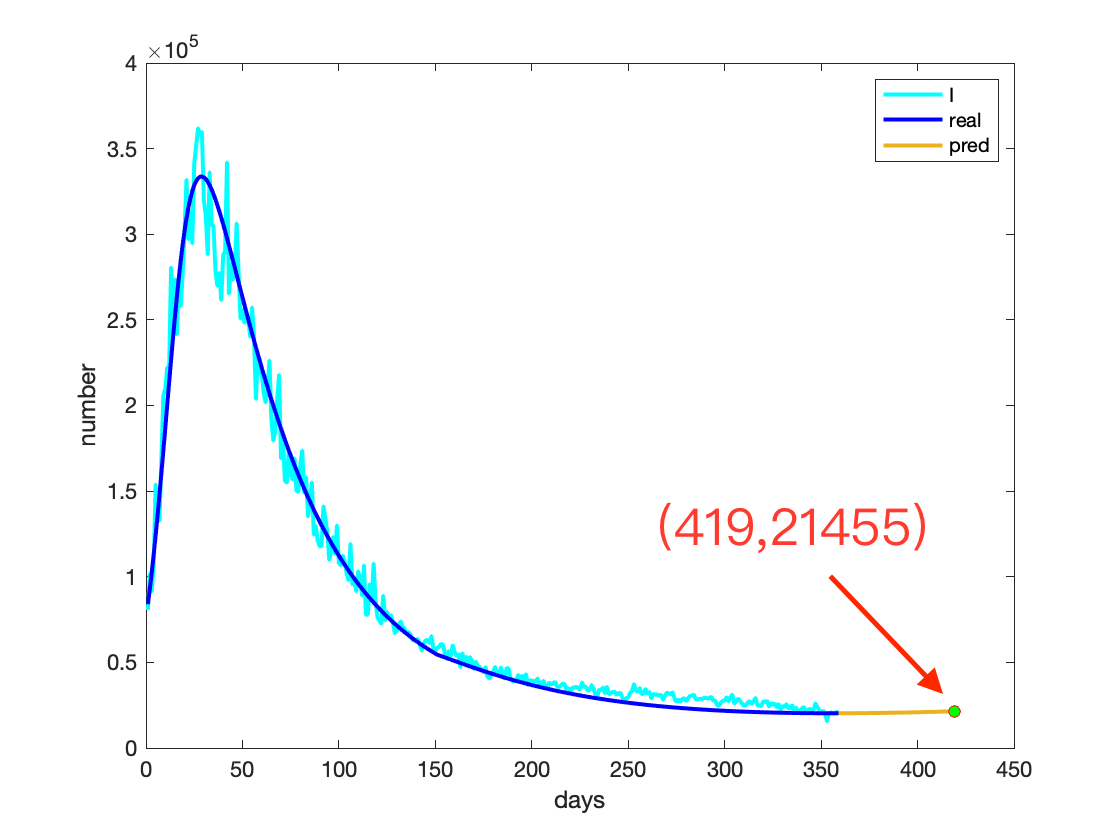
\includegraphics[width=\textwidth]{SRIS3.jpg}
		
	\end{subfigure}
	\caption{The actual outcome }\label{fig:subfigures}
\end{figure}

So,As you can see from the graph above, the model fits pretty well, with Wordle's projected number of visitors Tweeting on March 1:\textbf{21455}







\subsubsection{The number of users in Hard Mode analysis}

\begin{figure}[htbp]
	\centering
	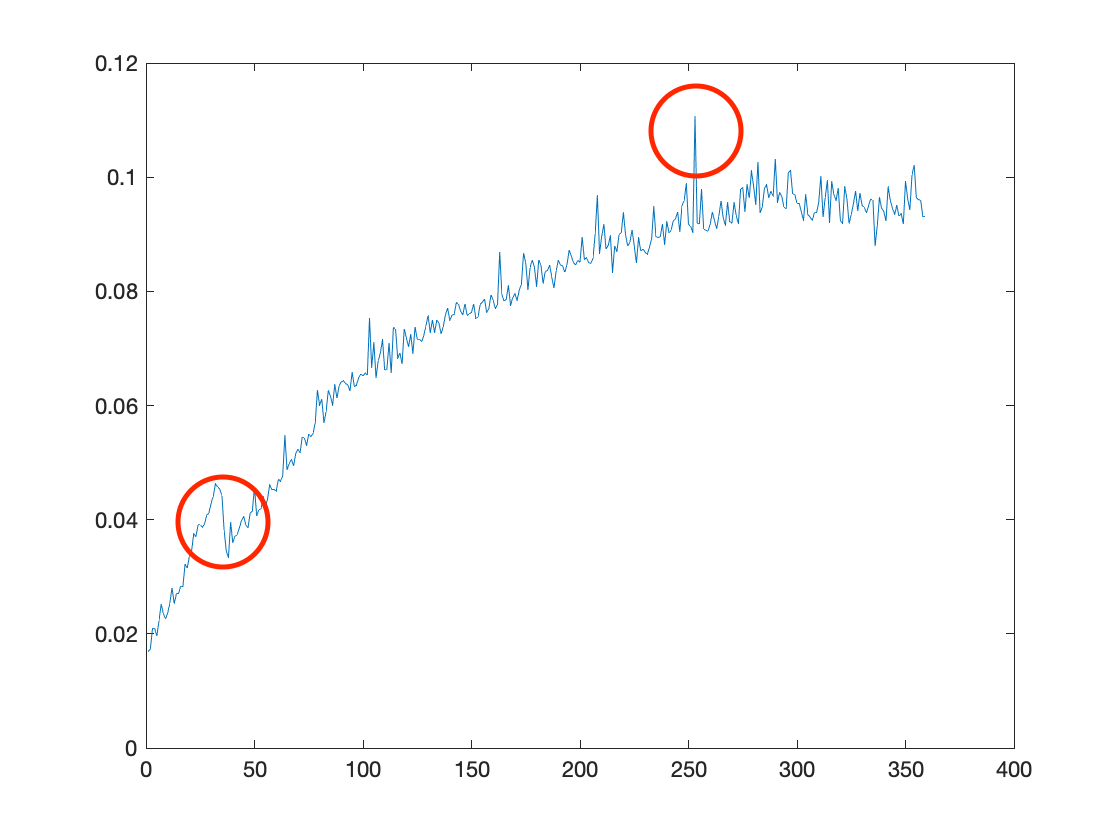
\includegraphics[width=0.9\textwidth]{HardMode1.png}
	\caption{The number of users in Hard Mode}\label{fig:result}
\end{figure}


About play difficult patterns percentage, its variation as above, it can be seen that as time goes on, the number of people play hard mode is rising gradually. This is logical, because as you play Wordle, you will become more proficient and will be eager to challenge the more difficult modes.


As for the two of these mutations, our interpretation is as follows:According to our review of wordle tags on Twitter, people tend to think they are lucky when they spend less time guessing, so people tend not to play hard mode when they hope to be lucky today (because it will take more time to guess). The first point is Valentine's Day, people hope to get lucky. So fewer people will play hard Mode.
As for the second, that Halloween is near, the day with 48\% of people don't guess, the more people may be due to falling back, or you want to pull people launching model of psychological encourages others to try hard.But no matter how hard we try to explain, we still can't give our own proper reason, we checked the official Wrodle Twitter post, and found that the above two points are actually \textbf{Wrong} data! We made the correction and then analyzed the change trend.

\clearpage



\begin{figure}[htbp]
	
	\begin{subfigure}[b]{.5\textwidth}
		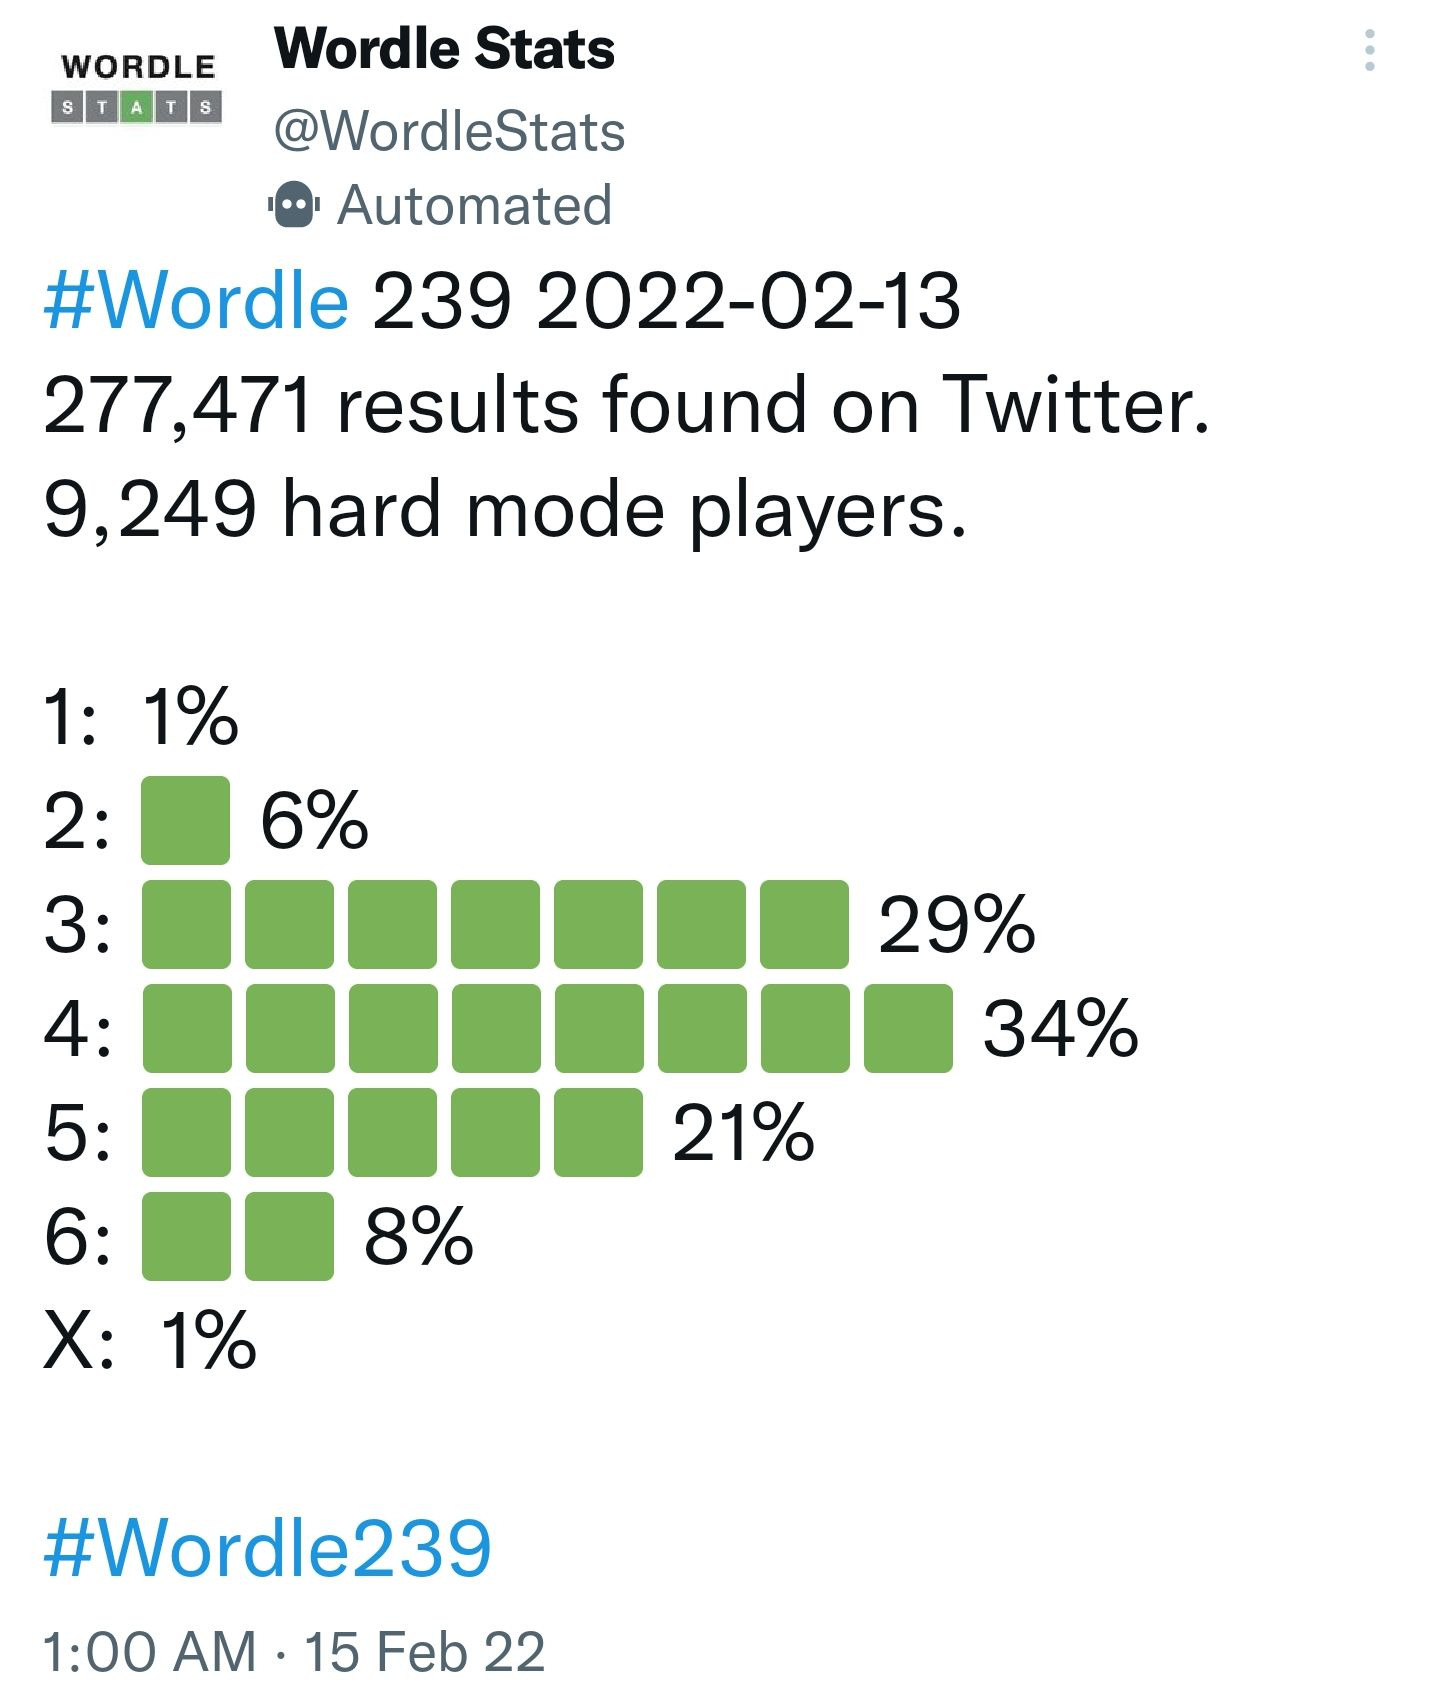
\includegraphics[width=\textwidth]{HM1.jpg}
		\caption{The data on 13 Feb 22}\label{subfig:left}
	\end{subfigure}
	\begin{subfigure}[b]{.455\textwidth}
		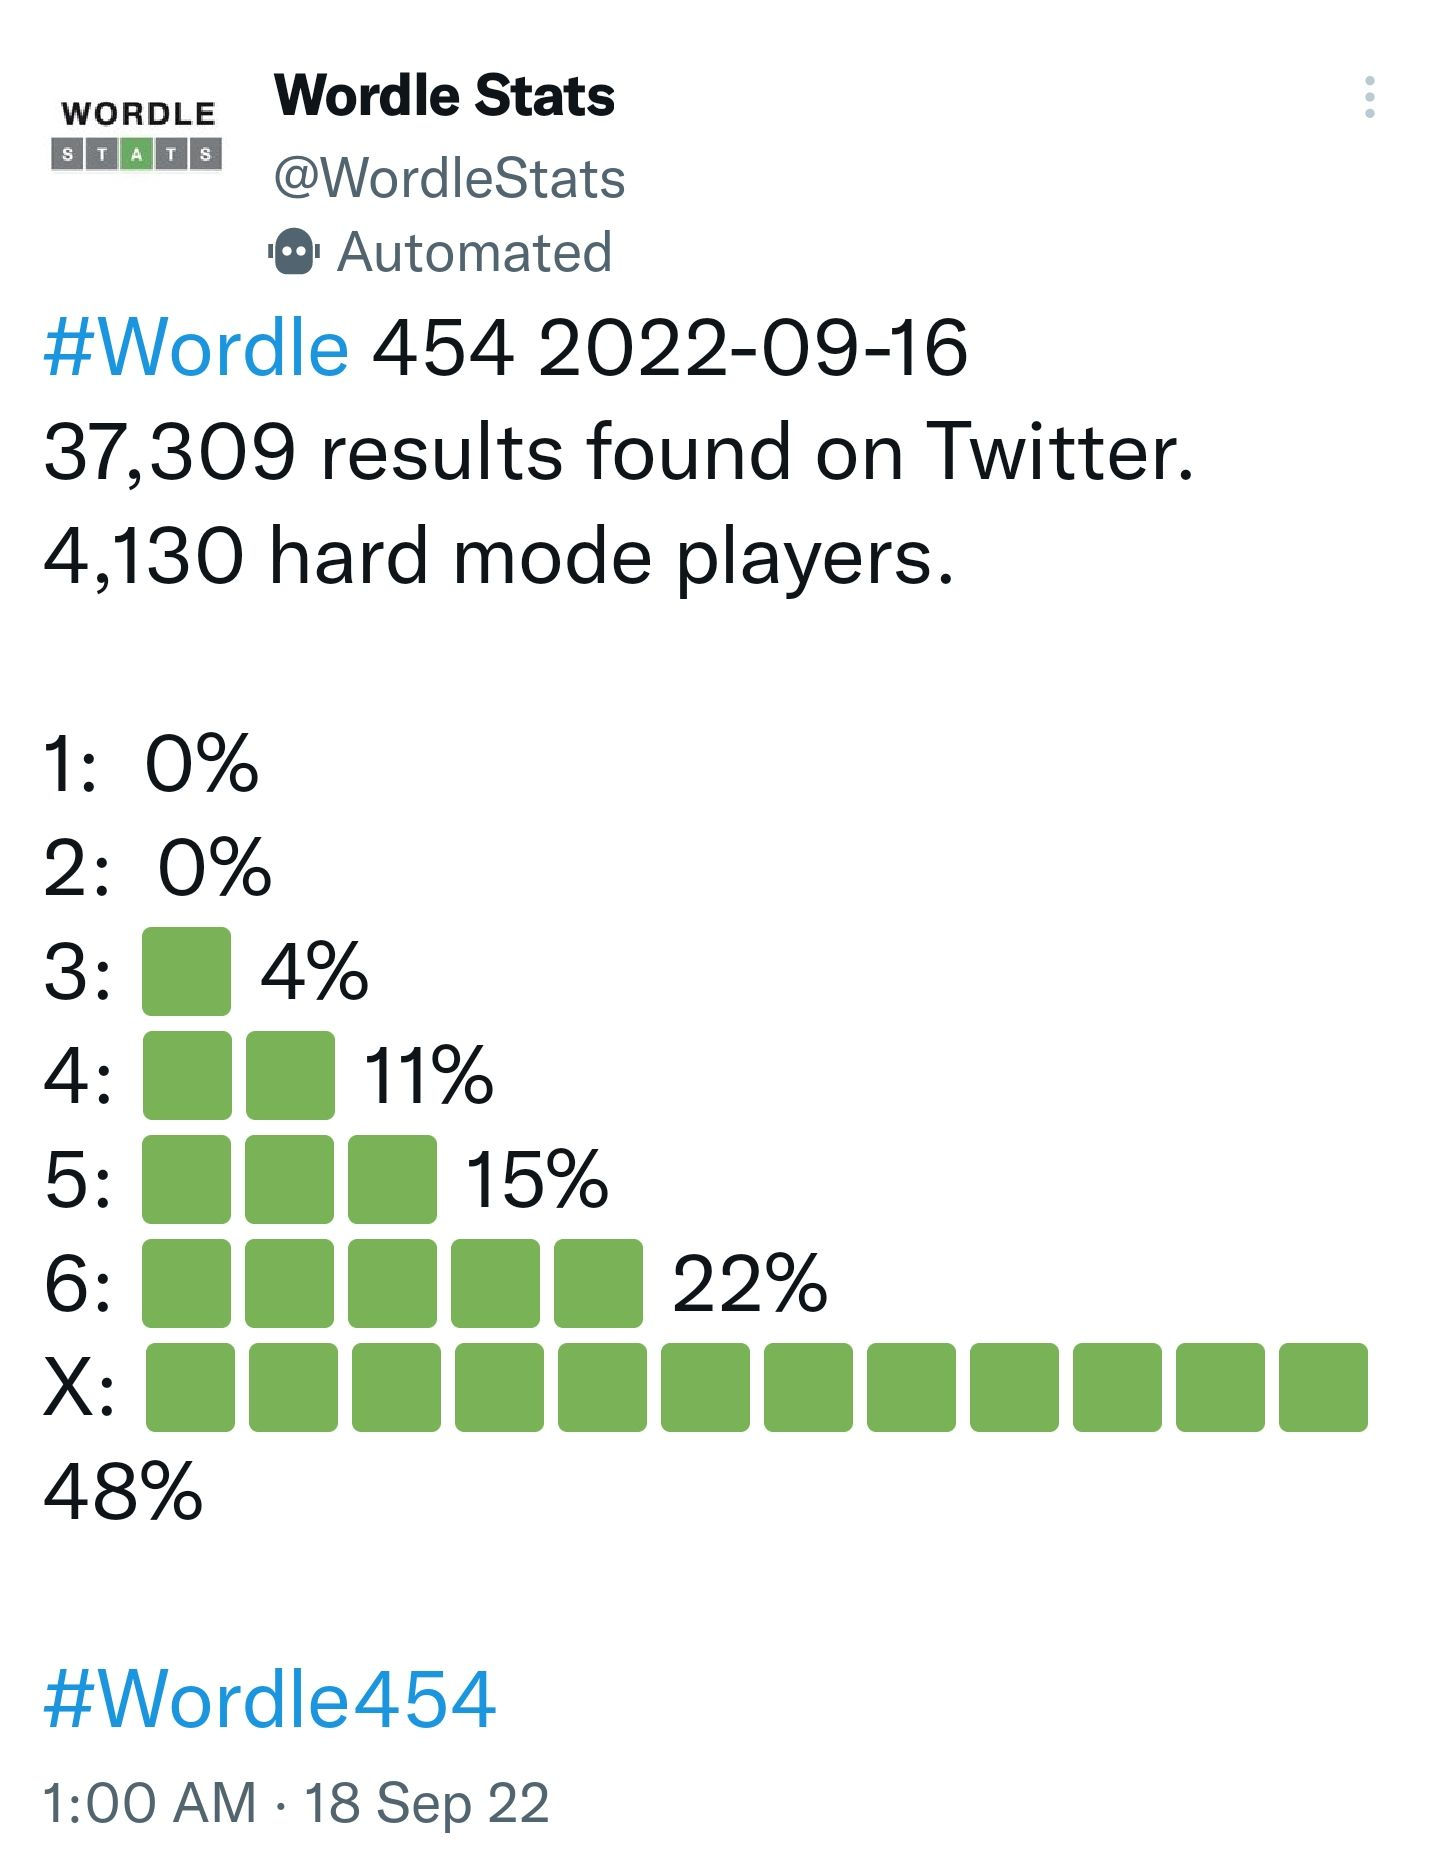
\includegraphics[width=\textwidth]{HM2.jpg}
		\caption{The data on 16 Sep 22}\label{subfig:right}
	\end{subfigure}
	\caption{The abruptly changed data \cite{2}}\label{fig:subfigures}
\end{figure}



\subsubsection{Disadvantages of Model 1}


The curve function fitting only uses the part behind the data, which makes the curve have certain limitations. We sacrifice some things for accuracy.
In the SIRS Model, there are still some differences between the model we obtained and the problem in practice. For example, the spread of social networks is not exactly the same as that of infectious diseases.
\subsection{Model 2}
\subsubsection{Basic information of Model 2}
The model established for the second question and the third question is basically the same. All the words are scored, and all the scores are divided into 5 sections, respectively (0-0.25), (0.25-0.3), (0.3-0.37), (0.37-0.7) (0.7-1.0) (in this way, the score sections are divided according to the number of samples).For each period of normal distribution fittingThe EERIE was analyzed, its score was obtained, its interval was found, and the proportion of 1,2,3,4,5,6, X was calculated by applying the corresponding normal distribution formula


Uncertainty: Different grading scales for words may conflict with each other
Confidence is expressed by correlation coefficient. 0.5604.

\begin{equation}
	\large f(x) =  a_1\cdot e^{-\frac{x-b_1}{c_1}^2}
\end{equation}

$$Coefficient(Confidence bounds: 95\%)$$


\begin{table}[!htbp]
	\begin{center}
		\caption{Gauss 1}
		\begin{tabular}{cl}
			\toprule
			\multicolumn{1}{m{3cm}}{\centering Symbol}
			&\multicolumn{1}{m{8cm}}{\centering Range or Value}\\
			\midrule
			$ a1=31.94  $&   \qquad\qquad \qquad Range (28.13, 35.74)\\
			$ b1=3.892  $&   \qquad\qquad \qquad Range(3.72, 4.064)\\
			$ c1=1.771  $&   \qquad\qquad \qquad Range(1.527, 2.015)\\
			$ SSE $&   \qquad\qquad\qquad\qquad 11.09\\
			$ R^2 $&   \qquad\qquad\qquad\qquad 0.9869\\
			$  Adjusted\quad  R^2 $&   \qquad\qquad\qquad\qquad 0.9804\\
			$ RMSE$&   \qquad\qquad\qquad\qquad1.665\\
			\bottomrule
		\end{tabular}\label{tb:notation}
	\end{center}
\end{table}


\begin{table}[!htbp]
	\begin{center}
		\caption{Gauss 2}
		\begin{tabular}{cl}
			\toprule
			\multicolumn{1}{m{3cm}}{\centering Symbol}
			&\multicolumn{1}{m{8cm}}{\centering Range or Value}\\
			\midrule
			$ a1=32.42  $&   \qquad\qquad \qquad Range (28.25, 36.6)\\
			$ b1=3.976   $&   \qquad\qquad \qquad Range (3.792, 4.16)\\
			$ c1=1.752  $&   \qquad\qquad \qquad Range(1.491, 2.013)\\
			$ SSE $&   \qquad\qquad\qquad\qquad13.22\\
			$ R^2 $&   \qquad\qquad\qquad\qquad 0.9852\\
			$  Adjusted\quad  R^2 $&   \qquad\qquad\qquad\qquad 0.9778\\
			$ RMSE$&   \qquad\qquad\qquad\qquad1.818\\
			\bottomrule
		\end{tabular}\label{tb:notation}
	\end{center}
\end{table}


\begin{table}[!htbp]
	\begin{center}
		\caption{Gauss 3}
		\begin{tabular}{cl}
			\toprule
			\multicolumn{1}{m{3cm}}{\centering Symbol}
			&\multicolumn{1}{m{8cm}}{\centering Range or Value}\\
			\midrule
			$ a1=33.68  $&   \qquad\qquad \qquad Range (29.85, 37.51)\\
			$ b1=4.039  $&   \qquad\qquad \qquad Range (3.883, 4.195)\\
			$ c1=1.682  $&   \qquad\qquad \qquad Range (1.461, 1.903)\\
			$ SSE $&   \qquad\qquad\qquad\qquad 10.69\\
			$ R^2 $&   \qquad\qquad\qquad\qquad0.989\\
			$  Adjusted\quad  R^2 $&   \qquad\qquad\qquad\qquad 0.9836\\
			$ RMSE$&   \qquad\qquad\qquad\qquad1.635\\
			\bottomrule
		\end{tabular}\label{tb:notation}
	\end{center}
\end{table}


\begin{table}[!htbp]
	\begin{center}
		\caption{Gauss 4}
		\begin{tabular}{cl}
			\toprule
			\multicolumn{1}{m{3cm}}{\centering Symbol}
			&\multicolumn{1}{m{8cm}}{\centering Range or Value}\\
			\midrule
			$ a1=33.99  $&   \qquad\qquad \qquad Range  (29.83, 38.15)\\
			$ b1=4.193  $&   \qquad\qquad \qquad Range  (4.026, 4.36)\\
			$ c1=1.67   $&   \qquad\qquad \qquad Range  (1.434, 1.907)\\
			$ SSE $&   \qquad\qquad\qquad\qquad 12.54\\
			$ R^2 $&   \qquad\qquad\qquad\qquad 0.9875\\
			$  Adjusted\quad  R^2 $&   \qquad\qquad\qquad\qquad 0.9812\\
			$ RMSE$&   \qquad\qquad\qquad\qquad 1.771\\
			\bottomrule
		\end{tabular}\label{tb:notation}
	\end{center}
\end{table}


\begin{table}[!htbp]
	\begin{center}
		\caption{Gauss 5}
		\begin{tabular}{cl}
			\toprule
			\multicolumn{1}{m{3cm}}{\centering Symbol}
			&\multicolumn{1}{m{8cm}}{\centering Range or Value}\\
			\midrule
			$ a1=33.71  $&   \qquad\qquad \qquad Range    (30.37, 37.04)\\
			$ b1=4.539  $&   \qquad\qquad \qquad Range    (4.402, 4.675)\\
			$ c1=1.692    $&   \qquad\qquad \qquad Range  (1.498, 1.887)\\
			$ SSE $&   \qquad\qquad\qquad\qquad8.131\\
			$ R^2 $&   \qquad\qquad\qquad\qquad 0.9918\\
			$  Adjusted\quad  R^2 $&   \qquad\qquad\qquad\qquad 0.9877\\
			$ RMSE$&   \qquad\qquad\qquad\qquad  1.426\\
			\bottomrule
		\end{tabular}\label{tb:notation}
	\end{center}
\end{table}

\begin{figure}[htbp]
	
	\begin{subfigure}[b]{.33\textwidth}
		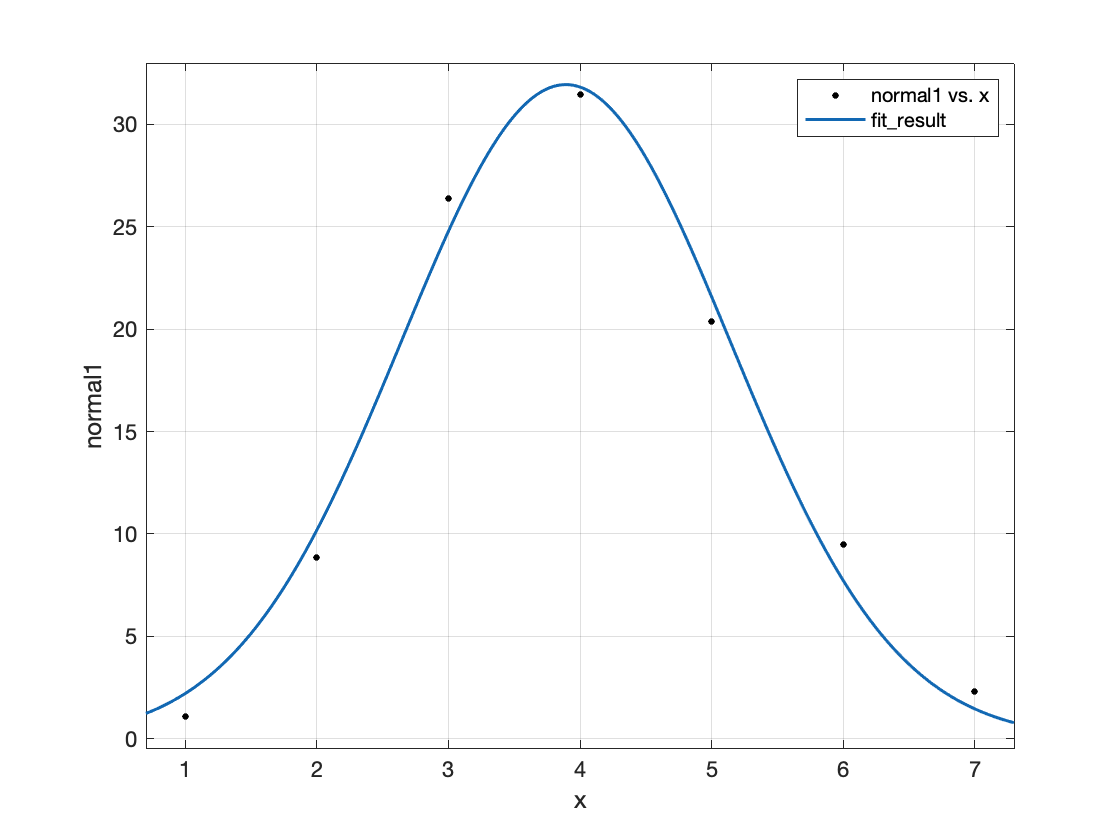
\includegraphics[width=\textwidth]{normal1.png}
		\caption{Normal1}\label{subfig:left}
	\end{subfigure}
	\begin{subfigure}[b]{.33\textwidth}
		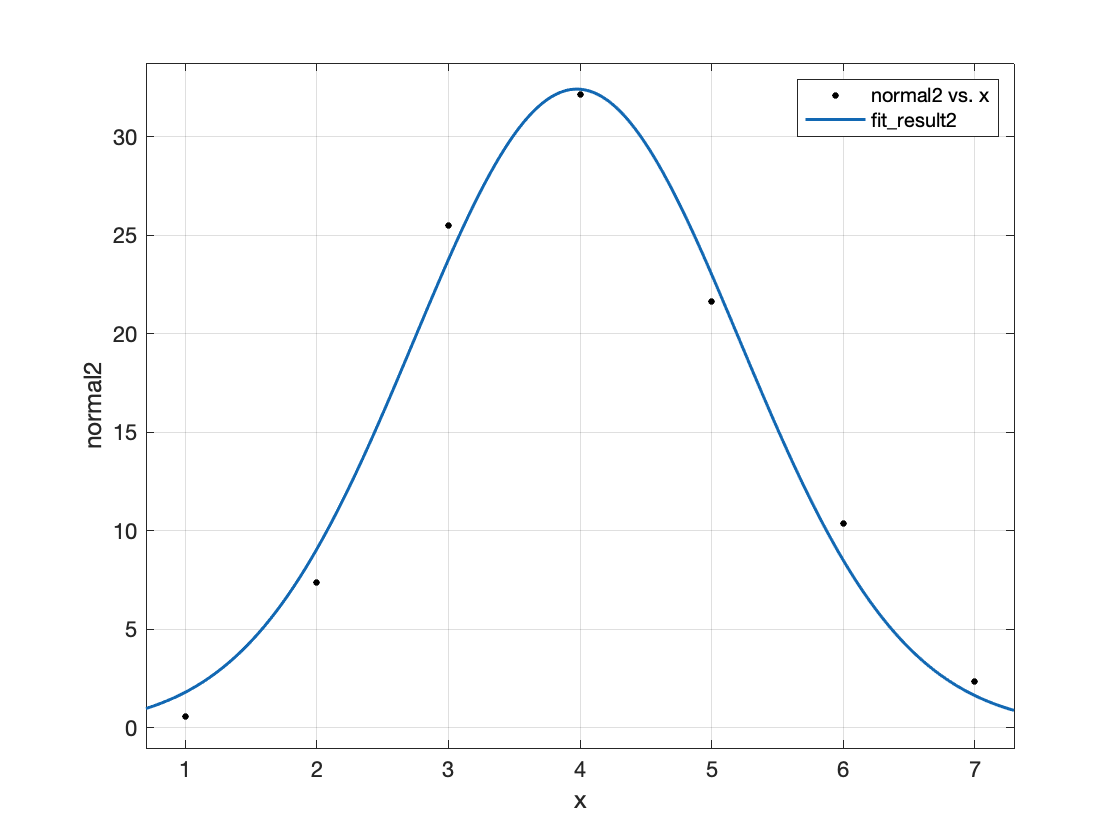
\includegraphics[width=\textwidth]{normal2.png}
		\caption{Normal2}\label{subfig:right}
	\end{subfigure}
   \begin{subfigure}[b]{.33\textwidth}
        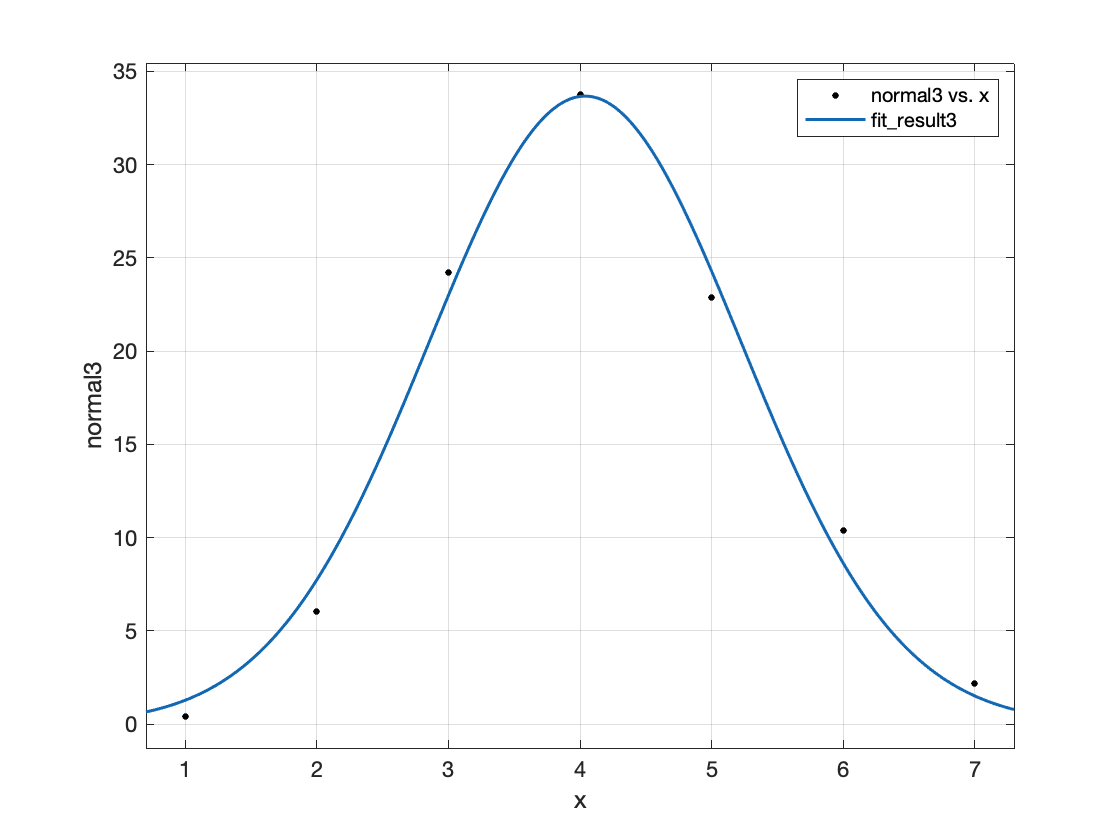
\includegraphics[width=\textwidth]{normal3.png}
	    \caption{Normal3}\label{subfig:right}
    \end{subfigure}

\begin{subfigure}[b]{.33\textwidth}
		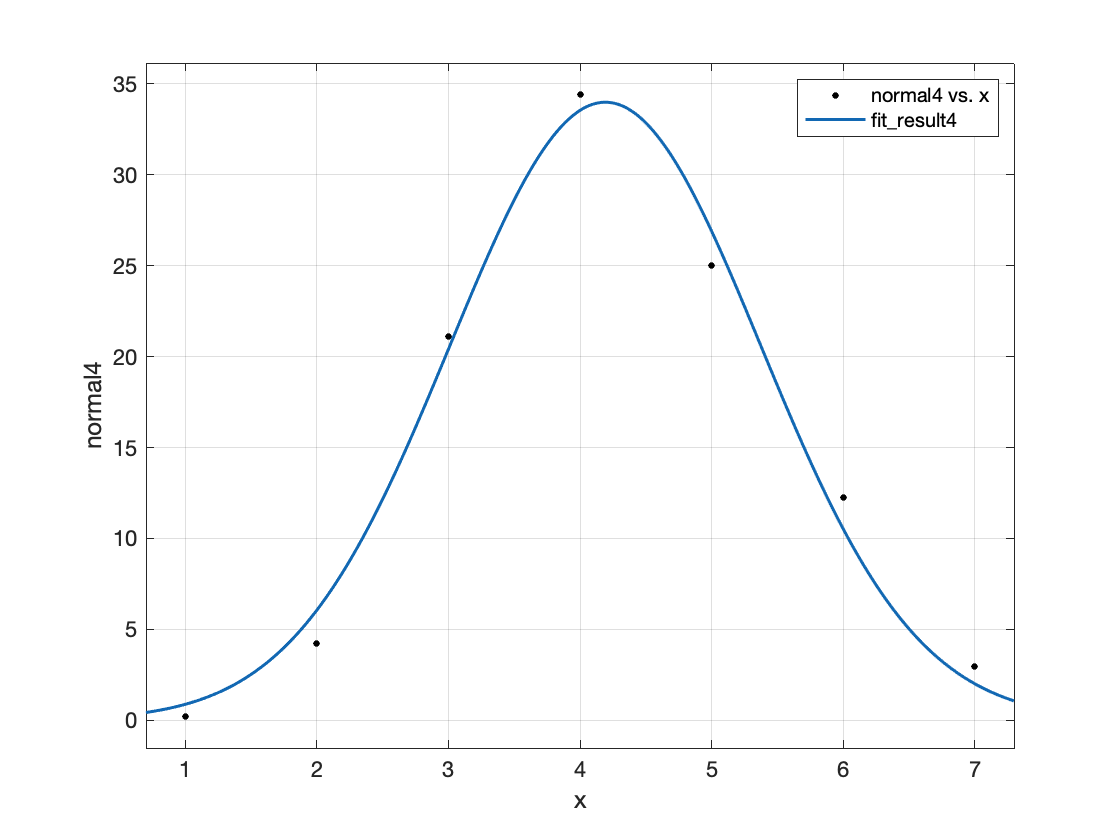
\includegraphics[width=\textwidth]{normal4.png}
		\caption{Normal4}\label{subfig:left}
	\end{subfigure}
	\begin{subfigure}[b]{.33\textwidth}
		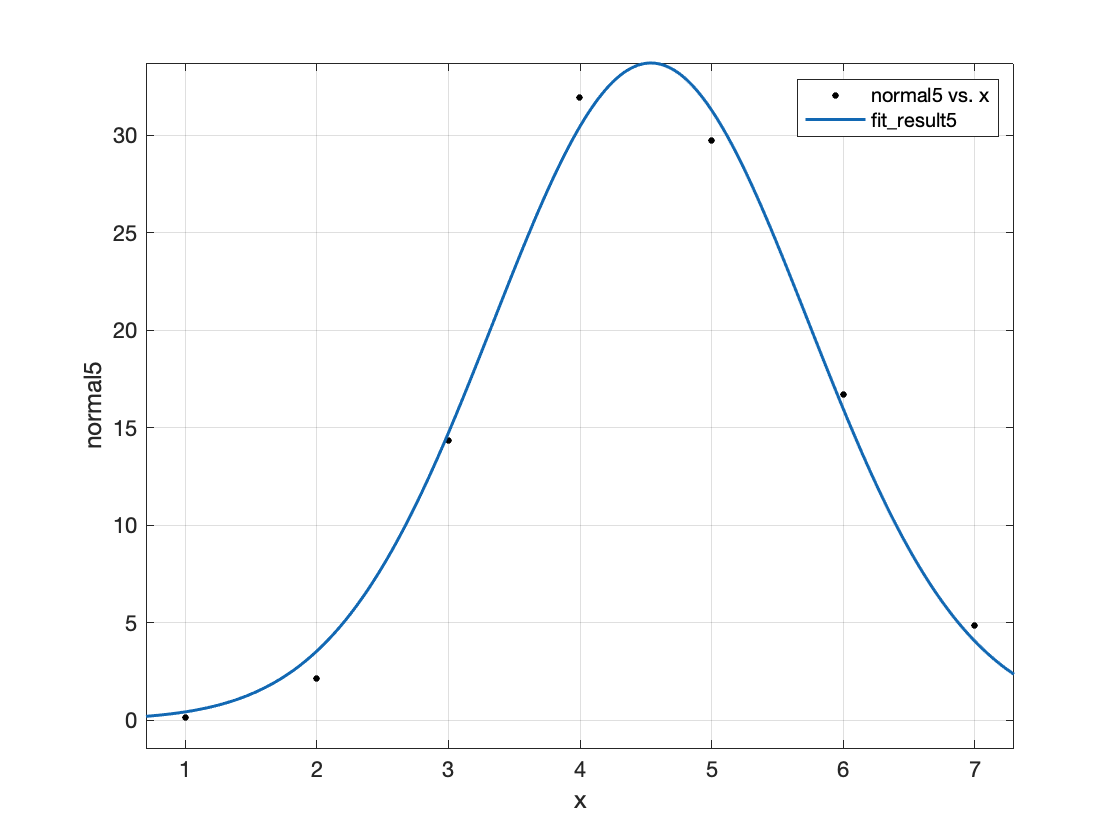
\includegraphics[width=\textwidth]{normal5.png}
		\caption{Normal5}\label{subfig:right}
	\end{subfigure}

	\caption{Normal 1-5 }\label{fig:subfigures}
\end{figure}

\clearpage

\subsubsection{The conclusion of Model 2}
EERIE then uses the above evaluation system to get his relevant indicators.
For the analysis of the percentage of times of each word, we believe that it is a discrete point conforming to a normal distribution, and only a few cases do not conform to it. Its distribution is just like human height and weight, which should obey the normal distribution.
From there, we looked at the percentage distribution for each word, and we found some correlation. For example, the more difficult the word, the higher the mean of the normal distribution function (corresponding to the number of guesses required to guess the word).
Our idea is to divide the 359 words in the system into five levels according to the uniform number of sample values through the evaluation system in our second question. The corresponding difficulty coefficient evaluation score is (0-0.25), (0.25-0.30), (0.30-0.37), (0.37-0.7), (0.7-1.0) (divided according to the number of samples, each section of grade has the relatively same amount of words). Of course, the percentage distribution of all words in each difficulty interval is normal, and their mean and variance should be similar.
We evaluate the percentage of each degree of a word by fitting the data normal distribution function.


Easy, Relatively easy, Normal, Relatively hard, Hard

\begin{figure}[htbp]
	\centering
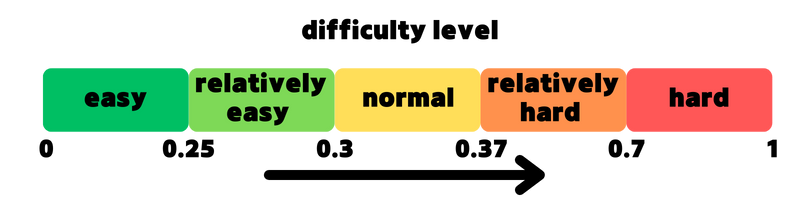
\includegraphics[width=0.9\textwidth]{Level.png}
\caption{Diffculity Level}\label{fig:result}
\end{figure}

\begin{table}[!htbp]
	\begin{center}
		\caption{The Difficulty Factor of 6 words}
		\begin{tabular}{cl}
			\toprule
			\multicolumn{1}{m{3cm}}{\centering Word}
			&\multicolumn{1}{m{8cm}}{\centering Difficulty factor}\\
			\midrule
			$ third  $&   \qquad\qquad \qquad\qquad 0.2366\\
			$ mummy  $&   \qquad\qquad \qquad\qquad 0.8689\\
			$ apply   $&   \qquad\qquad\qquad \qquad 0.6693\\
			$ leave $&   \qquad\qquad\qquad\qquad0.5530\\
			$ class $&   \qquad\qquad\qquad\qquad0.6116\\
			$ other $&   \qquad\qquad\qquad\qquad 0.0794\\
			$EERIE $&   \qquad\qquad\qquad\qquad 0.6046\\
			\bottomrule
		\end{tabular}\label{tb:notation}
	\end{center}
\end{table}

So,the difficulty level of EERIE is is \textbf{relative hard}

\subsubsection{Disadvantages of Model 2}
When Model2 evaluates word attributes, it lacks more attributes, which makes our evaluation system have certain limitations and cannot analyze this practice from a more comprehensive perspective, thus increasing the uncertainty of prediction.



\clearpage
\subsection{Model 3}
\begin{figure}[htbp]
	\centering
	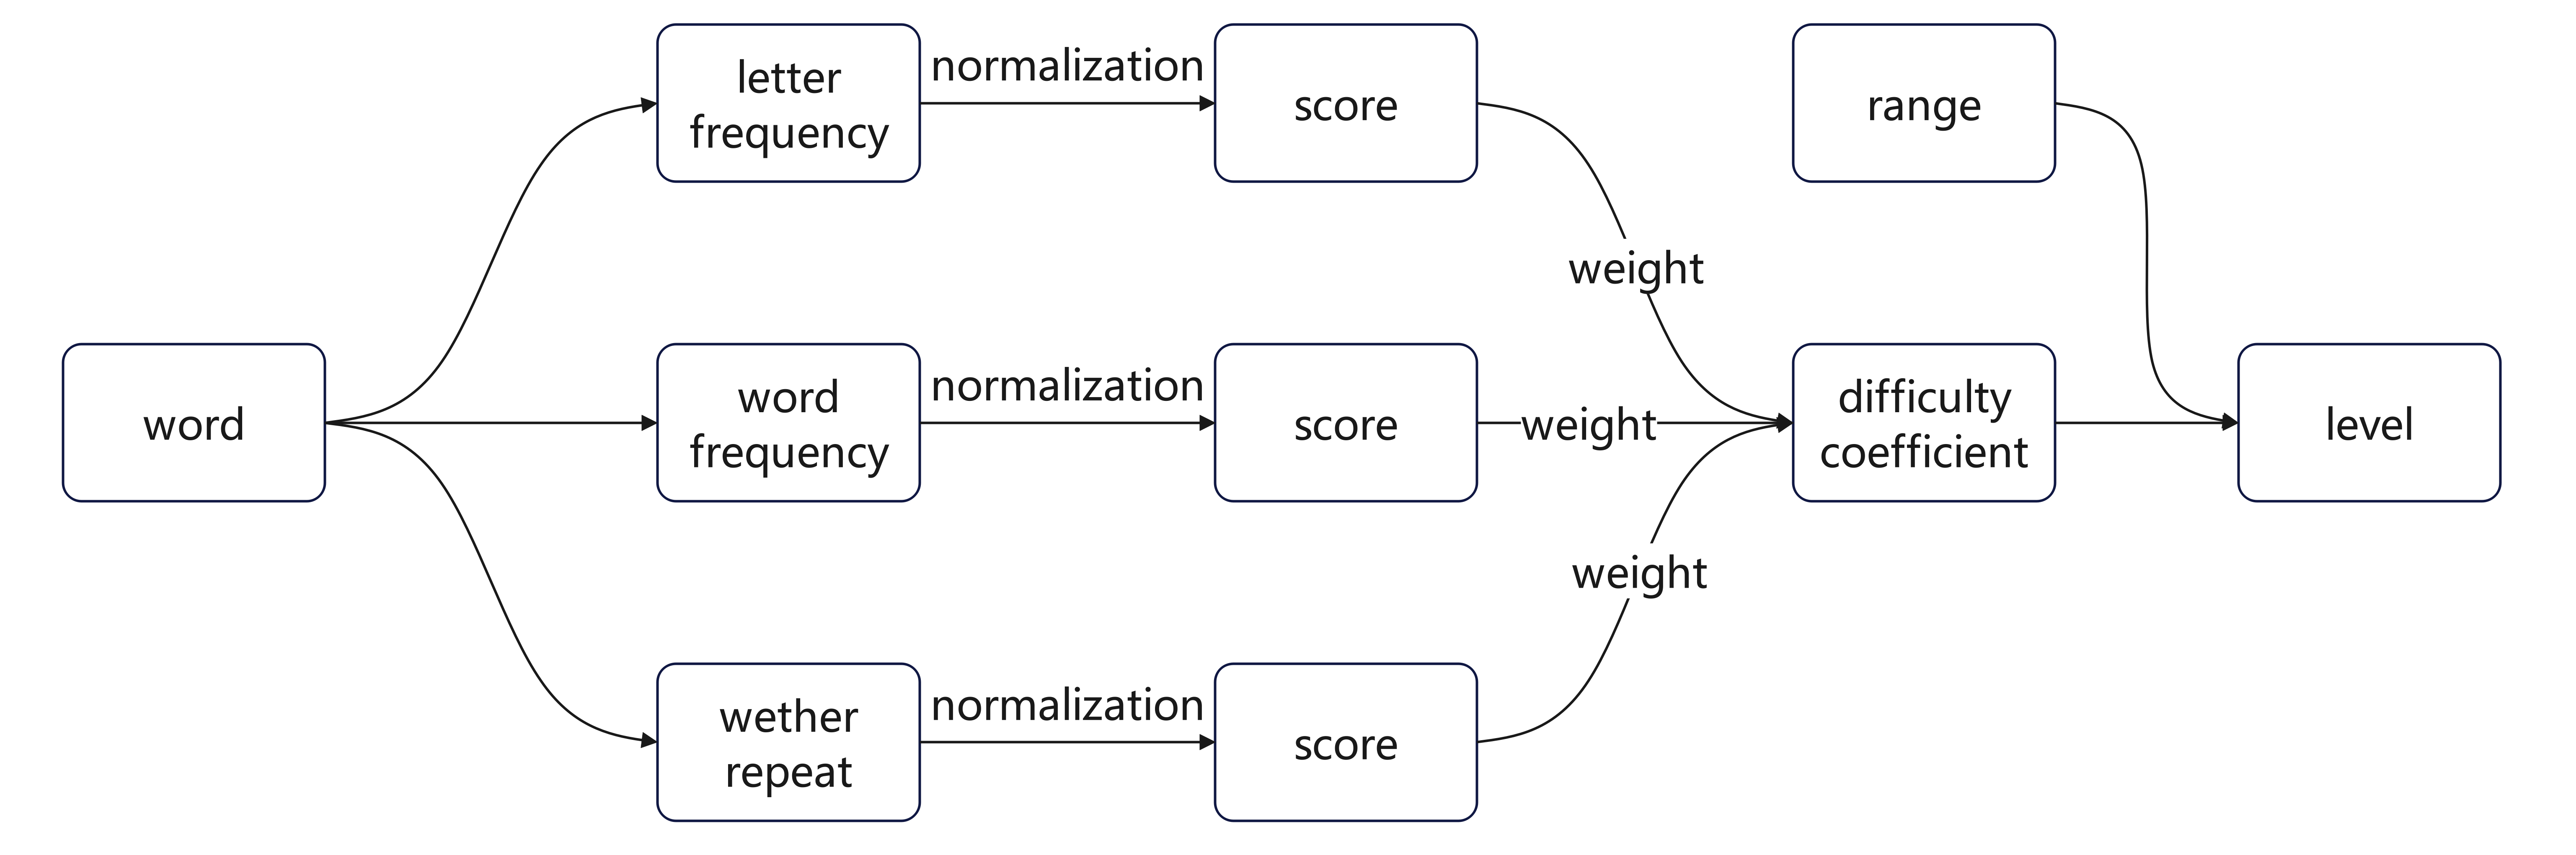
\includegraphics[width=1.0\textwidth]{process.png}
	\caption{ The attritube of words}\label{fig:result}
\end{figure}


Select the attributes of the word: (1) Letter frequency; (2) Word frequency (3) Whether there are repeated letters; (4) The number of vowels; (5) More than three repetitions; (6) Whether the beginning word is a vowel sound; (7) Whether the ending is a vowel sound; (8) Continuous repetition.
Since each attribute has a different dimension, normalization is used to group all data into the same dimension between 0 and 1
After we analyzed all the attributes, we selected a few important ones for analysis
(1) Letter frequency
Using all the letters in issue 359 as a sample to estimate the frequency of each of the five letter words,
A table of letter frequencies
Add up the five letter frequencies for each word to represent how common the letters in that word are


Use linear normalization:

\begin{equation}
	x' = \frac{x-min(x)}{max(x)-min(x)}
\end{equation}

\begin{figure}[htbp]
	\centering
	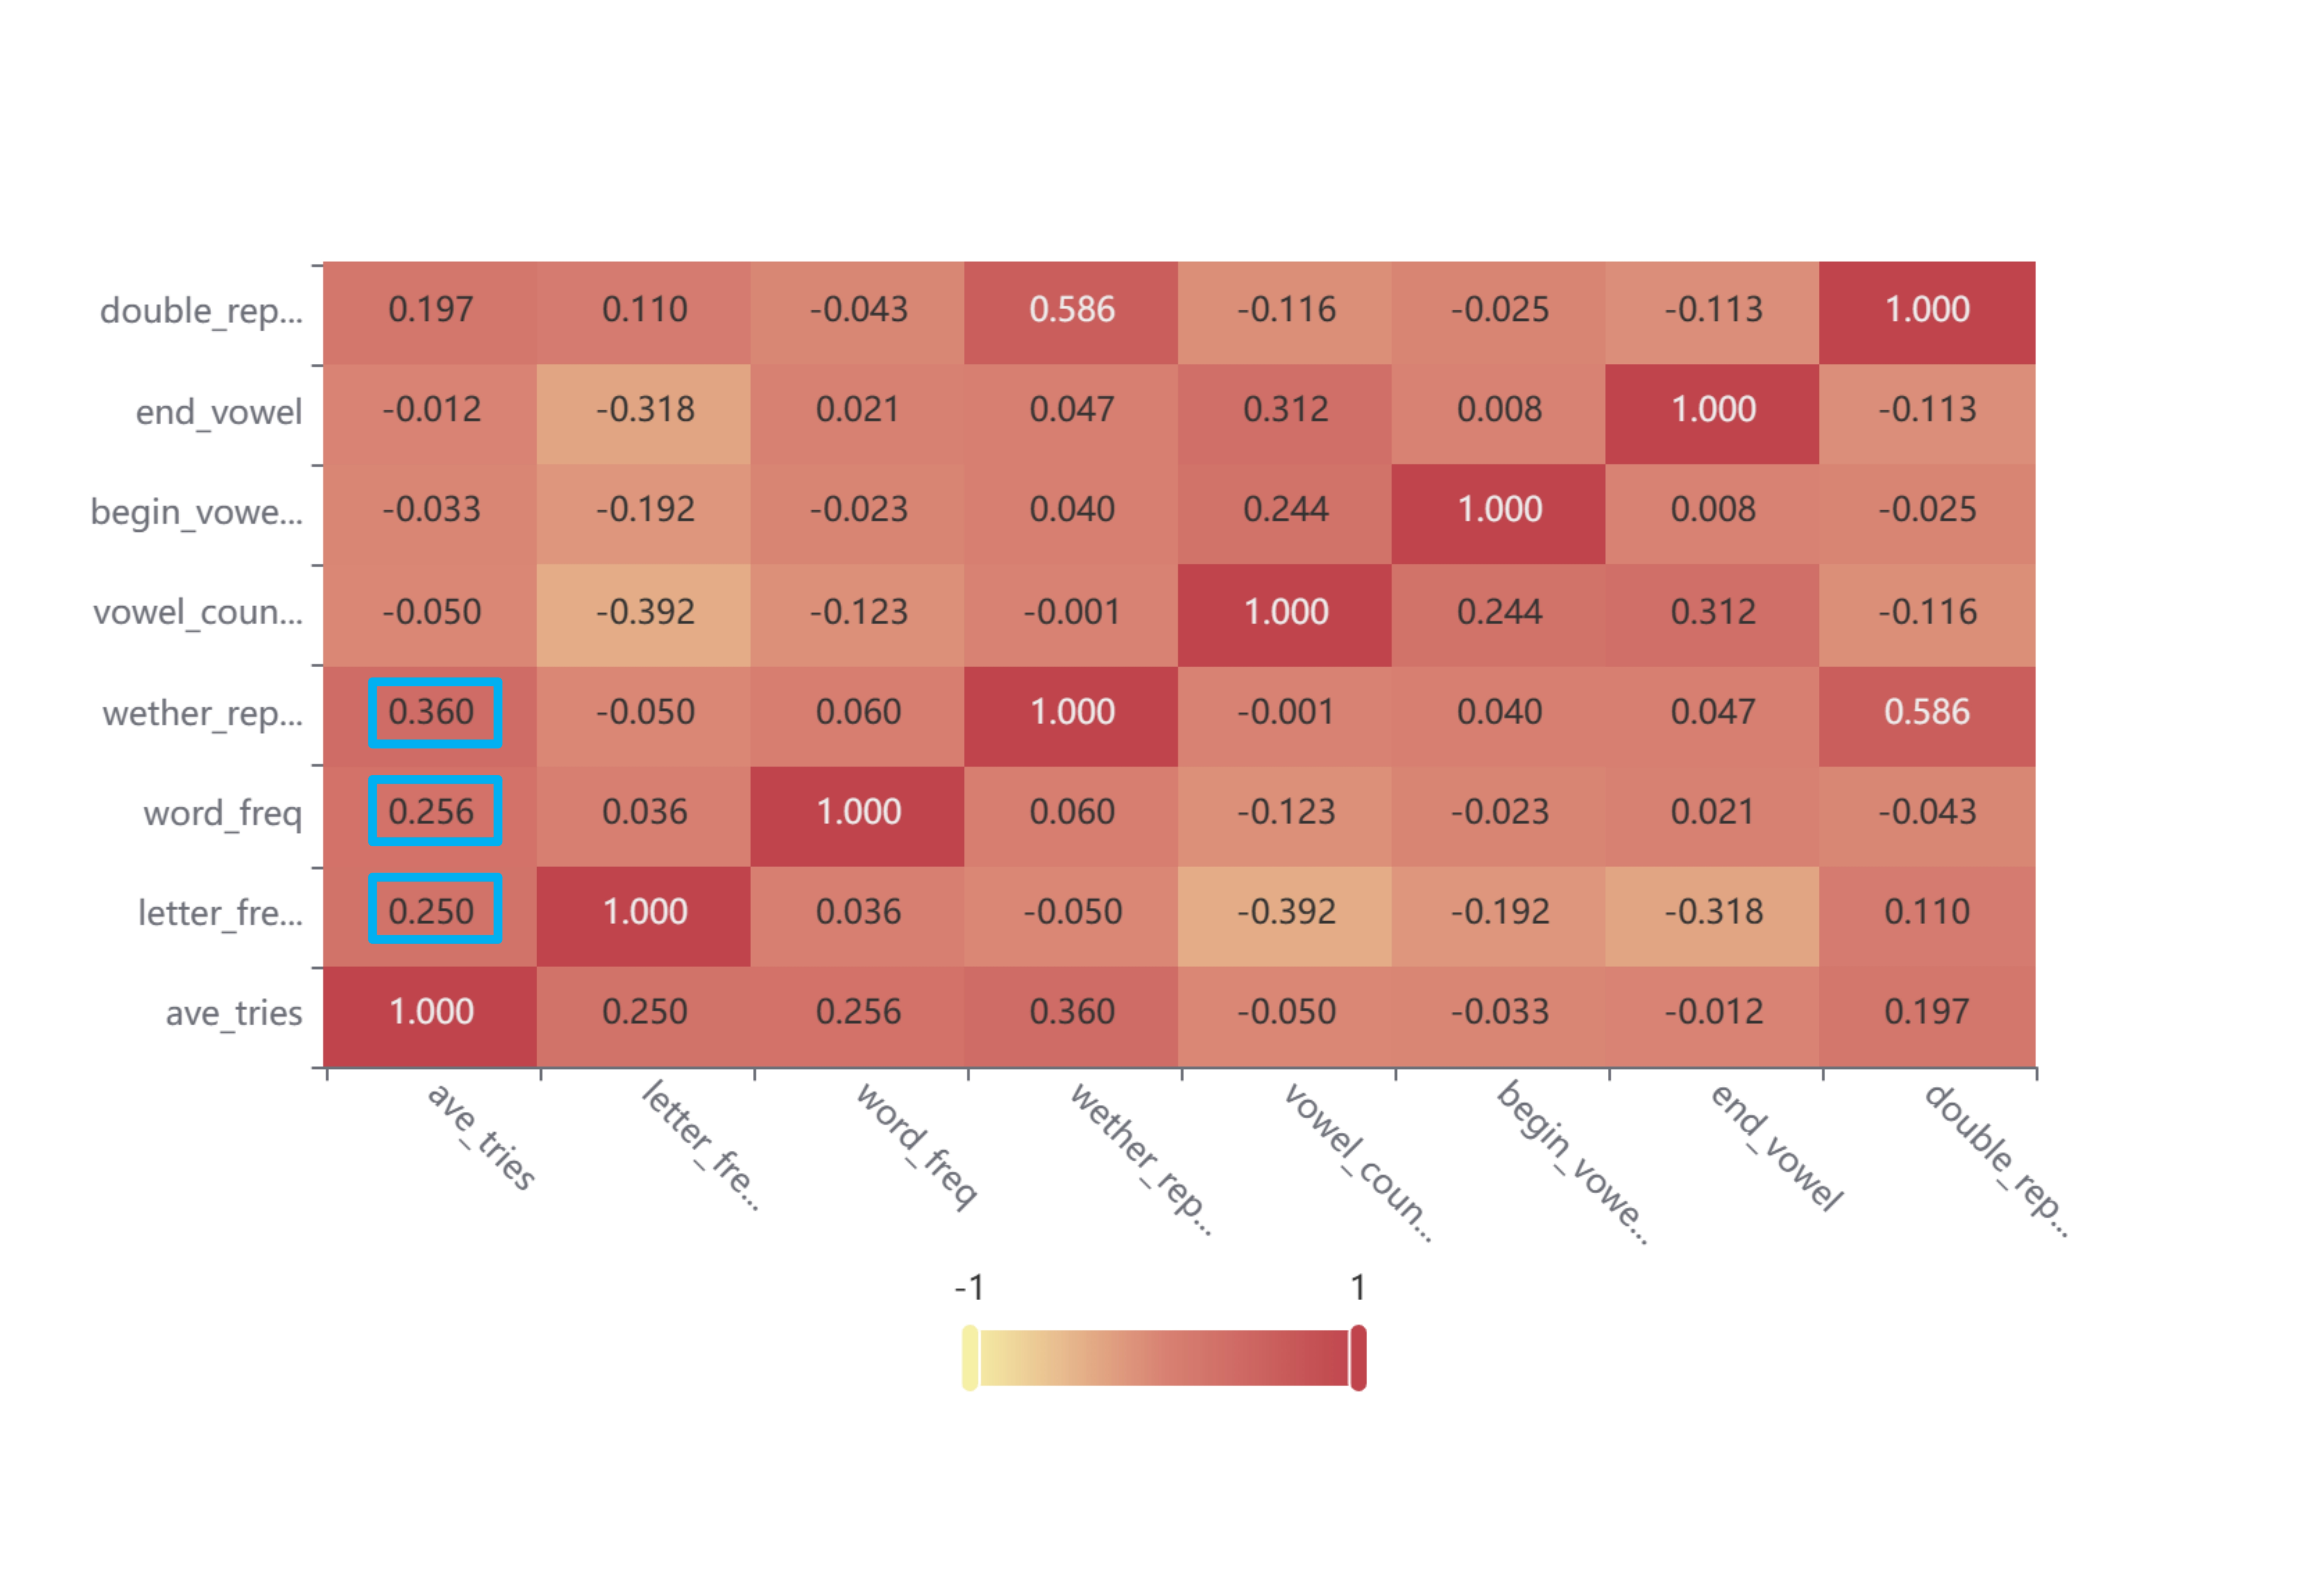
\includegraphics[width=1.0\textwidth]{RED1.jpg}
	\caption{ The attritube of words}\label{fig:result}
\end{figure}



Normalize the letter frequencies of all words to a range of 0 to 1
(2) Word frequency: Find the frequency of corresponding words from kaggle database\cite{3} , and use logarithmic normalization and then linear normalization to make the frequency of words fall into the range of 0-1
(3),(5),(6),(7),(8) are all 0,1 distribution so they don't need to be normalized
(4) Uniform normalization is also adopted
The average number of words: the weighted method is adopted to calculate the average number of words. Seven times and above are identified as seven times. (Add the formula and calculate an average number of times for example) The uniform normalization method is also adopted to normalize the average number of times
Then the average number of guesses equal the difficulty of the word.
Calculate covariance coefficients between (1)-(7) and difficulty to represent their relationship.



The correlation between word frequency, letter frequency and repetition is relatively large. The three attributes of words are weighted to get the weight, and then the evaluation system is established. After evaluating all the words, the cocorrelation coefficient between our evaluation system and the average number of times can reach 0.5, which is a very effective improvement.

\begin{figure}[htbp]
	\centering
	\includegraphics[width=0.7\textwidth]{Letter1.png}
	\caption{Word Cloud }\label{fig:result}
\end{figure}

\begin{figure}[htbp]
	\centering
	\includegraphics[width=0.9\textwidth]{Letter2.png}
	\caption{The frequceny of letters}\label{fig:result}
\end{figure}





% 长表格示例,更多用法请参考 longtable 宏包文档
% 以下环境及对应参数可实现表格内的自动换行与表格的自动断页
% 您也可以选择自行载入 tabularx 宏包,并通过 X 参数指定对应列自动换行






% 子图(多图并列)示例,更多用法请参考 subfigure 宏包文档
% 如果您只希望几张图并列,不需要额外的 caption,那么在 figure 环境中
% 连续插入总宽度不超过 \textwidth 的多个 \includegraphics 命令即可
\subsubsection{Disadvantages of Model 3}

The Model3 evaluation system is divided into five difficulty levels, but when adopting classification, we adopt an almost average number of interval words instead of uniform word difficulty coefficient scoring. Although this makes words have greater universality in this evaluation system, when words are in easy and hard difficulty respectively, their difficulty scores differ too much, which has a certain chance.

\section{Uncertainties and shortcomings of the overall model}

\subsection{Uncertainty:}
a. Background uncertainty of game words
We only analyzed the letter attributes of the words and their frequency of use, while the meaning of the words themselves and the scenes in which they were used could not be intuitively obtained. The lack of analysis of this point in our word evaluation system made the data more uncertain.


b. Subjective uncertainty in games
There is no guarantee that the evolution of games is constant, and game patterns and activities may change over time, making our data obsolete. Or there may be some other objective factor that changes the game dramatically.


c. Uncertainty of participants
We only build the model from the level of data, not from the character of the people, the mood of the people who participate in the game. Also, tweeting is a heterogeneous behavior that doesn't take into account the direct impact between the person tweeting and the person playing the game
\subsection{Disadvantages:}
a. When we process data, we use a relatively simple normalization method, which may not be able to better highlight the characteristics of data.


b. When we use the evaluation system to determine the weights represented by different data, we ignore the mutual influence, which makes our evaluation system adulterated with uncertainty factors.

\section{Some interesting things}
During this modeling process, we found a number of interesting things. These things are accidental discoveries during the modeling and programming process. Although they do not have a great impact on the final result, we still believe that these thoughts and discoveries can play a great role and arouse our interest in modeling.


1. What we think are the best first words
After counting the frequency of words, it was no surprise that e topped the list. While we analyzed the difficulty ratings of existing words, we also kept playing the game Wordle. We think we can guess words using words made up of letters that appear more frequently. Because the first guess is a blind guess, we don't have any information until we type the first word. And when we guess words made up of letters that appear more frequently, we have a greater chance of getting yellow or even green tiles, providing ample information for a second guess. The first six letters are e, a, r, o, t, l, so we have the greatest chance of getting more useful information if we guess the word ALERT as the first word. ALERT is a word that has a high frequency per word. A similar word is STORE EARTH.


2. According to data analysis, when the number of people tweeting after playing Wordle game becomes stable, the number of people with difficulty accounts for about 10\% of the total number of people, which generally does not change with the change of word attributes. Using the simple universal game Wordle, we can get a rough estimate of the population from this sample, which we can use to estimate the overall personality traits of the population. People who choose the difficult mode can be understood as those who are willing to face difficulties and dare challenges to a certain extent and context. In all groups, the number of people who are willing to take risks accounts for about 10\%.


% 以下为信件/备忘录部分,不需要可自行去掉
% 如有需要可将整个 letter 环境移动到文章开头或中间
% 请在第二个花括号内填写标题,如「信件」(Letter)或「备忘录」(Memorandum)

\begin{letter}{Letter}
	\begin{flushleft}  % 左对齐环境,无首行缩进
		\textbf{To:} Puzzle Editor of the New York Times\\
		\textbf{From:} Team 2306372 of 2023 MCM\\
		\textbf{Date:} Feb 20, 2023\\
		\textbf{Subject:} Analysis of Wordle and future advice 
	\end{flushleft}
	\headrule
	\begin{flushleft}
		Dear Puzzle Editor of the New York Times
	\end{flushleft}
	
	In this letter, we want to congratulate you first that Wordle has gone viral at the beginning of year 2022 under your editing. After receiving the data from MCM we do some analyses on this popular game and found some interesting results. Also our team want to offer you some advice for the future operation of the game. The detailed information is as follow:
	
	Firstly,  The game's simplicity, coupled with its addictive nature, led to it becoming a viral sensation on social media platforms.
	
	However, since its peak popularity, the number of daily tweets and overall engagement surrounding Wordle has declined. Despite this, the percentage of users opting to play the game in hard mode has increased. Hard mode in Wordle increases the number of letters in the word to six or seven and decreases the number of attempts allowed to five or four.
	
	This trend in user behavior indicates that while the novelty of the game may have worn off, users are still interested in playing, but they are seeking more challenging options to keep the game fresh and exciting. Therefore, to maintain and potentially increase user engagement, the game's operations team can introduce new game modes with more challenging options.
	
	For example, they could add a game mode where players have to guess a seven or eight-letter word in three attempts or less, or a mode where they must guess a word with a specific set of letters. Additionally, the team could also consider adding a multiplayer feature, where players can compete against each other to guess the word in the shortest amount of time.
	
	Continuously updating and improving Wordle with new features and game modes will help keep users engaged and maintain the game's popularity in the long run. By giving players more options and challenges, Wordle can continue to be a fun and addictive game for years to come.
	
	Secondly, We highly recommend your team to add our grading system to the game. So a player can have a brief idea that the word he or she guess today is a simple one or a hard one by telling them like:"you just guess a word which is harder than xx\% of all words in history", which can improve players' the sense of achievement, making them stick to the game.
	
	Lastly, you team can use our model developed in problem 2 to predict the distribution of the word chosen by you, our team think that a relative similar distribution each day can greatly improve the playing experience of Wordle.
	
	That's all of our analyses and suggestion to you. As a team hired by New York Times, our data is limited, however our models for the 3 problems above are proved to be effective on prediction and evaluate. Your team can do further analyses based on them. We sincerely hope that the Wordle will have a promising future.
\end{letter}



% 参考文献,此处以 MLA 引用格式为例
\begin{thebibliography}{99}
\bibitem{1} Compartmental models in epidemiology-WikiPedia, from \url{https://en.wikipedia.org/wiki/Compartmental_models_in_epidemiology}
\bibitem{2} WordleStats' post from \url{https://twitter.com/WordleStats}
\bibitem{3} \url{https://www.kaggle.com/datasets/rtatman/english-word-frequency}
\end{thebibliography}


% 以下为附录内容
% 如您的论文中不需要附录,请自行删除
\begin{subappendices}  % 附录环境

\section{Appendix: Program Codes}
Here are the program codes we used in our research.


% MATLAB 代码示例
\begin{lstlisting}[language=MATLAB, name={score_calc.m}]
score=(1:359);
for i=1:359
score(i)=0;
for j=1:5
for k=1:26
if letters(i,j)==lut(k,1)
score(i)=score(i)+double(lut(k,2));
end
end
end
end

\end{lstlisting}
\begin{lstlisting}[language=MATLAB, name={sort_letter_freq.m}]
words = char(words);
words = words(:);
rank= tabulate(words);
rank = sortrows(rank,-2);
\end{lstlisting}
\begin{lstlisting}[language=MATLAB, name={SEIR_test.m}]
figure;
[t,h] = ode45(@SEIR,(1:359),[0.2 0.8 0.05 0.05]); 
plot(t,h(:,1),'r');
hold on;
plot(t,h(:,2),'b');
plot(t,h(:,3),'m');
plot(t,h(:,4),'g');
plot(t,usernum./400000,'c');
title('SEIR')


function dy=SEIR(t,x)
beta = 0.5;         
gamma1 = 0.001;     
gamma2 = 0.005;      
alpha = 0.5;        
dy=[alpha*x(3) - gamma2*x(1);
-beta*x(1)*x(2);
beta*x(1)*x(2) - (alpha+gamma1)*x(3);
gamma1*x(3)+gamma2*x(1)];
end

function dy=SIRS(t,x)
beta = 0.7;      
gamma = 0.15;    
alpha = 0.15;    
dy=[beta*x(1)*x(2)-gamma*x(1);
-beta*x(1)*x(2)+alpha*x(3)
gamma*x(1) - alpha*x(3)];
end
\end{lstlisting}
\begin{lstlisting}[language=MATLAB, name={SIRS.m}]
I=84000;
R=00;
N=525000;
S=N-I;
gama=0.0017;%jiechuchuanran
t=1:419;
lemda2=0.152
for i=1:(size(t,2)-1)
lemda=0.152;
mu=0.020;%zhiyu
if i >150
lemda=-0.1/400*i+0.4
mu=-0.01/250+0.0155
end            
I(1+i)=I(i)+I(i)*(N-I(i)-R(i))*lemda2/N-mu*I(i);
S(1+i)=S(i)-lemda*I(i)*S(i)/N+gama*R(i);
R(1+i)=N-I(1+i)-S(1+i);
end
plot(t(1:359),usernum(1:359),'c',t(1:359),I(1:359),'blue','LineWidth',2);
xlabel('days')
ylabel('number')
hold on
plot(t(359:end),I(359:end),'LineWidth',2);
plot(419,21455,'ro-','MarkerFaceColor','g')
legend('I','real','pred')
mid=(usernum-I).^2;
disp(sum(mid(50:359)));
\end{lstlisting}

\end{subappendices}  % 附录内容结束

\end{document}  % 结束
